\documentclass[12pt,a4paper]{article}
\usepackage[a4paper, margin=0.8in, headheight=14pt]{geometry}
\usepackage{fontspec}
\usepackage{unicode-math}
\setmainfont{TeX Gyre Pagella}
\setmonofont[Scale=0.88]{TeX Gyre Cursor}
\setmathfont{Latin Modern Math}
\usepackage{xcolor}
\usepackage{colortbl}
\usepackage{titlesec}
\usepackage{enumitem}
\usepackage{tabularx}
\usepackage{booktabs}
\usepackage{array}
\usepackage{amsmath}
\usepackage{tikz}
\usetikzlibrary{shapes.geometric, arrows.meta, positioning, calc, fit, decorations.pathreplacing, decorations.pathmorphing}
\usepackage{tcolorbox}
\tcbuselibrary{skins, breakable}
\usepackage{hyperref}
\usepackage{fancyhdr}
\usepackage{graphicx}
\usepackage{microtype}
\hyphenpenalty=10000
\exhyphenpenalty=10000
\sloppy
\usepackage{caption}
\usepackage{setspace}
\usepackage{multirow}
\usepackage{tocloft}
\newcommand{\Q}[1]{\textbf{#1}\par\noindent\ignorespaces}
\definecolor{myred}{RGB}{196,30,58}
\definecolor{mydark}{RGB}{30,30,50}
\definecolor{mygreen}{RGB}{14,120,80}
\definecolor{myteal}{RGB}{0,130,140}
\definecolor{myamber}{RGB}{180,100,0}
\definecolor{mypurple}{RGB}{100,30,160}
\definecolor{mygray}{RGB}{246,247,249}
\definecolor{mgframe}{RGB}{180,185,200}
\definecolor{watermark}{RGB}{145,150,170}
\definecolor{hdrred}{RGB}{250,232,235}
\definecolor{hdrgreen}{RGB}{220,244,233}
\definecolor{hdrteal}{RGB}{220,242,244}
\definecolor{hdramber}{RGB}{253,242,215}
\definecolor{hdrpurple}{RGB}{238,228,255}
\definecolor{hdrgray}{RGB}{238,240,245}
\definecolor{rowalt}{RGB}{250,251,253}

\titleformat{\section}{\large\bfseries\color{myred}}{\thesection.}{0.5em}{}[\vspace{1pt}{\color{myred}\rule{\linewidth}{0.8pt}}]
\titleformat{\subsection}{\normalsize\bfseries\color{myteal}}{\thesubsection}{0.5em}{}
\titlespacing*{\section}{0pt}{18pt}{7pt}
\titlespacing*{\subsection}{0pt}{11pt}{4pt}
\setlength{\parindent}{0pt}
\setlength{\parskip}{4pt}
\renewcommand{\cfttoctitlefont}{\large\bfseries\color{myred}}
\renewcommand{\cftaftertoctitle}{\par\noindent{\color{myred}\rule{\linewidth}{0.8pt}}}
\setlength{\cftbeforetoctitleskip}{0pt}
\setlength{\cftaftertoctitleskip}{6pt}
\renewcommand{\cftsecfont}{\normalsize\bfseries\color{mydark}}
\renewcommand{\cftsecpagefont}{\normalsize\bfseries\color{mydark}}
\renewcommand{\cftsecleader}{\cftdotfill{\cftdotsep}}
\setlength{\cftbeforesecskip}{7pt}
\renewcommand{\cftsubsecfont}{\small\color{mydark}}
\renewcommand{\cftsubsecpagefont}{\small\color{mydark}}
\setlength{\cftbeforesubsecskip}{3pt}
\setlength{\cftsubsecindent}{1.4em}
\renewcommand{\cftpartfont}{\normalsize\bfseries\color{myteal}}
\renewcommand{\cftpartpagefont}{\normalsize\bfseries\color{myteal}}
\setlength{\cftbeforepartskip}{14pt}
\renewcommand{\arraystretch}{1.45}
\setlength{\tabcolsep}{6pt}
\arrayrulecolor{mydark}
\newcolumntype{B}[1]{>{\small\bfseries\raggedright\arraybackslash}m{#1}}
\newcolumntype{C}[1]{>{\centering\arraybackslash}m{#1}}
\newcolumntype{Y}{>{\small\raggedright\arraybackslash}X}
\renewcommand{\tabularxcolumn}[1]{m{#1}}
\newcommand{\currmodule}{Module 1}
\pagestyle{fancy}
\fancyhf{}
\fancyhead[L]{\small\color{myred}\textbf{PE-EC703A}\;\color{mydark}--- Embedded System}
\fancyhead[R]{\small\color{myteal}\textbf{\currmodule\ Notes}}
\fancyfoot[C]{\small\color{mydark}\thepage}
\fancyfoot[R]{\small\color{watermark}\textit{\copyright\ Biraj}}
\renewcommand{\headrulewidth}{0.5pt}
\renewcommand{\footrulewidth}{0.3pt}

\hypersetup{colorlinks=true, linkcolor=myteal, urlcolor=myteal,
  pdfauthor={Biraj Sarkar},
  pdftitle={PE-EC703A --- Combined Notes}}

\tcbset{
  tikzbox/.style={
    colback=mygray, colframe=mgframe, boxrule=0.6pt, arc=4pt,
    left=8pt, right=8pt, top=6pt, bottom=6pt,
    colbacktitle=mgframe, coltitle=mydark,
    fonttitle=\small\bfseries
  },
  defbox/.style={
    colback=hdrgreen, colframe=mygreen, boxrule=0.8pt, arc=4pt,
    left=9pt, right=9pt, top=6pt, bottom=6pt,
    colbacktitle=mygreen, coltitle=white,
    fonttitle=\small\bfseries
  },
  formulabox/.style={
    colback=hdrteal, colframe=myteal, boxrule=0.8pt, arc=4pt,
    left=9pt, right=9pt, top=7pt, bottom=7pt,
    colbacktitle=myteal, coltitle=white,
    fonttitle=\small\bfseries
  },
  examplebox/.style={
    colback=hdramber, colframe=myamber, boxrule=0.8pt, arc=4pt,
    left=9pt, right=9pt, top=6pt, bottom=6pt,
    colbacktitle=myamber, coltitle=white,
    fonttitle=\small\bfseries
  },
  masonbox/.style={
    colback=hdrpurple, colframe=mypurple, boxrule=0.8pt, arc=4pt,
    left=9pt, right=9pt, top=6pt, bottom=6pt,
    colbacktitle=mypurple, coltitle=white,
    fonttitle=\small\bfseries
  },
  exambox/.style={
    colback=hdrpurple, colframe=mypurple, boxrule=1pt, arc=5pt,
    left=10pt, right=10pt, top=8pt, bottom=8pt,
    colbacktitle=mypurple, coltitle=white,
    fonttitle=\bfseries,
    breakable, title after break={\textbf{Frequently Asked / Viva Questions (contd.)}}}
}
\tcbset{after={\color{black}}}

\tikzset{
  block/.style={rectangle, draw=myteal, fill=hdrteal,
    text width=2.4cm, align=center, minimum height=0.95cm,
    font=\small, rounded corners=3pt, line width=0.7pt},
  redblock/.style={rectangle, draw=myred, fill=hdrred,
    text width=2.4cm, align=center, minimum height=0.95cm,
    font=\small, rounded corners=3pt, line width=0.7pt},
  netnode/.style={rectangle, draw=myteal, fill=hdrteal,
    text width=1.5cm, align=center, minimum height=0.8cm,
    font=\small, rounded corners=3pt, line width=0.7pt},
  sumjunc/.style={circle, draw=myamber, fill=hdramber,
    minimum size=0.62cm, font=\small, line width=0.8pt},
  snode/.style={circle, draw=mypurple, fill=hdrpurple,
    minimum size=0.55cm, font=\footnotesize, line width=0.7pt},
  arrow/.style={-Stealth, thick, color=mydark},
  redarrow/.style={-Stealth, thick, color=myred},
  line/.style={thick, color=mydark}
}

\newcommand{\modulestart}[2]{%
  \clearpage
  \renewcommand{\currmodule}{Module #1}%
  \phantomsection
  \addcontentsline{toc}{part}{Module #1: #2}%
  \setcounter{section}{0}%
  \begin{center}
    \vspace*{1.0cm}
    {\Huge\bfseries\color{myred} Module #1}\\[10pt]
    {\Large\bfseries\color{mydark} #2}\\[10pt]
    {\color{myred}\rule{0.55\linewidth}{1.2pt}}
  \end{center}
  \vspace{14pt}
}
\begin{document}

\thispagestyle{empty}
\vspace*{1.0cm}
\begin{center}
  {\Huge\bfseries\color{myred} PE-EC703A}\\[10pt]
  {\LARGE\bfseries\color{mydark} Embedded System}\\[20pt]
  {\color{myred}\rule{0.7\linewidth}{1.5pt}}\\[18pt]
  {\Large\color{myteal}\textbf{Combined Module Notes}}\\[8pt]
  {\large\color{mydark} Modules 1 -- 5}\\[40pt]
  {\normalsize\color{mydark} Semester VII \quad$\bullet$\quad 3L:0T:0P \quad$\bullet$\quad 3 Credits}\\[12pt]
  {\normalsize\color{mydark} CGEC \;$|$\; B.Tech ECE (2023--27)}\\[6pt]
  {\normalsize\color{mydark}\textit{Biraj Sarkar}}
\end{center}
\vspace{1.0cm}
\begin{center}
  \begin{tcolorbox}[colback=mygray, colframe=mgframe, boxrule=0.5pt, arc=3pt, width=0.85\linewidth]
    \centering\small\color{mydark}
    \textbf{Disclaimer / Study Guide Notice:}\\
    These are condensed \textbf{Short Notes} focusing on core theory, key formulas, block/circuit diagrams, and standard viva Q\&As for university exam revision. Exhaustive numerical practice problems and derivation edge cases are not covered. This serves as a quick-revision reference guide for students.
  \end{tcolorbox}
\end{center}
\vfill
\begin{center}{\small\color{watermark}\textit{Exam-Ready Notes}}\end{center}
\clearpage

\hypersetup{linkcolor=mydark}
\tableofcontents
\hypersetup{linkcolor=myteal}
\clearpage

% -- Module 1 -----------------------------------------------------------------
\modulestart{1}{What is an Embedded System?}

\section{What is an Embedded System?}
% ===============================================================================

An embedded system is a combination of hardware and software designed to perform a specific dedicated function within a larger system. Unlike general-purpose computers, embedded systems are purpose-built and optimized for a particular task.

\begin{tcolorbox}[defbox, title={\textbf{Embedded System --- Definition}}]
An \textbf{embedded system} is a dedicated computing system that is tightly integrated into the device it controls. It consists of a microprocessor or microcontroller, memory, I/O interfaces, and software (firmware) designed to perform one or more specific tasks --- often with real-time constraints and limited resources (power, memory, processing speed).
\end{tcolorbox}

\subsection{Key Characteristics}
\begin{itemize}[leftmargin=*, itemsep=3pt]
  \item \textbf{Single-function:} Designed to perform a specific task (e.g., engine control, temperature monitoring).
  \item \textbf{Real-time operation:} Must respond to events within strict time deadlines.
  \item \textbf{Resource-constrained:} Limited memory (RAM/ROM), processing power, and energy budget.
  \item \textbf{Reliability:} Must operate continuously and correctly, often without human intervention.
  \item \textbf{Embedded into a product:} The computing part is hidden inside a larger product (e.g., washing machine, car).
\end{itemize}

% ===============================================================================
\section{Embedded Processor in a System}
% ===============================================================================

\begin{tcolorbox}[defbox, title={\textbf{Embedded Processor}}]
An \textbf{embedded processor} is the central computational element of an embedded system. It can be a \textbf{microprocessor} (requires external memory and peripherals), a \textbf{microcontroller} (integrates CPU, memory, and peripherals on a single chip), a \textbf{DSP} (optimized for signal processing), or an \textbf{FPGA/ASIC} (for high-speed, custom logic).
\end{tcolorbox}

\subsection{Types of Embedded Processors}

\par\noindent
{\renewcommand{\arraystretch}{1.6}%
\begin{tabularx}{\linewidth}{|B{3.0cm}|Y|Y|}
\hline
\textbf{Processor Type} & \textbf{Description} & \textbf{Examples / Use} \\
\hline
\textbf{Microcontroller (MCU)} & CPU + RAM + ROM + I/O on one chip & 8051, PIC, ARM Cortex-M, AVR \\
\hline
\textbf{Microprocessor (MPU)} & CPU only; needs external memory and peripherals & Intel 8086, ARM Cortex-A \\
\hline
\textbf{DSP Processor} & Optimized for multiply-accumulate (MAC) operations & TMS320, SHARC \\
\hline
\textbf{FPGA / ASIC} & Reconfigurable / custom-designed logic fabric & Xilinx, Intel Altera \\
\hline
\textbf{SoC} & Entire system (CPU + GPU + memory + I/O) on one die & Qualcomm Snapdragon, Raspberry Pi SoC \\
\hline
\end{tabularx}}

% ===============================================================================
\section{Components of an Embedded System}
% ===============================================================================

An embedded system is made up of several hardware and software components that work together.

\begin{tcolorbox}[tikzbox, title={Components of an Embedded System}]
\centering
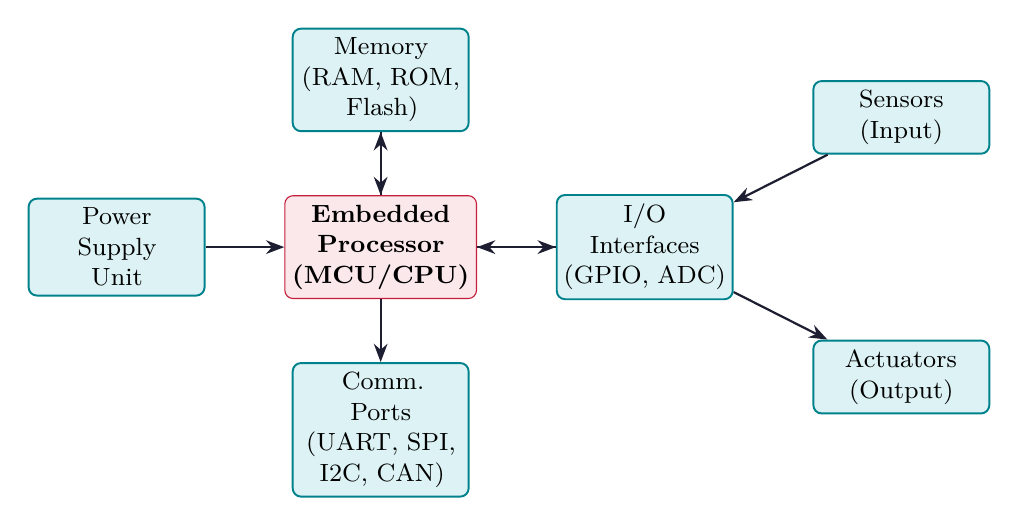
\begin{tikzpicture}[node distance=0.4cm and 0.7cm,
  sblock/.style={rectangle, draw=myteal, fill=hdrteal, text width=2.0cm,
    align=center, minimum height=0.85cm, font=\small,
    rounded corners=3pt, line width=0.7pt}]
  % Central MCU
  \node[rectangle, draw=myred, fill=hdrred, text width=2.2cm, align=center,
    minimum height=1.0cm, font=\small\bfseries, rounded corners=3pt] (mcu) {Embedded\\Processor\\(MCU/CPU)};
  % Surrounding blocks
  \node[sblock, above=0.8cm of mcu] (mem) {Memory\\(RAM, ROM,\\Flash)};
  \node[sblock, right=1.0cm of mcu] (io) {I/O\\Interfaces\\(GPIO, ADC)};
  \node[sblock, below=0.8cm of mcu] (comm) {Comm.\\Ports\\(UART, SPI,\\I2C, CAN)};
  \node[sblock, left=1.0cm of mcu] (pwr) {Power\\Supply\\Unit};
  \node[sblock, above right=0.5cm and 1.0cm of io] (sens) {Sensors\\(Input)};
  \node[sblock, below right=0.5cm and 1.0cm of io] (act) {Actuators\\(Output)};

  \draw[arrow] (mcu) -- (mem);
  \draw[arrow] (mem) -- (mcu);
  \draw[arrow] (mcu) -- (io);
  \draw[arrow] (io) -- (mcu);
  \draw[arrow] (mcu) -- (comm);
  \draw[arrow] (pwr) -- (mcu);
  \draw[arrow] (sens) -- (io);
  \draw[arrow] (io) -- (act);
\end{tikzpicture}
\end{tcolorbox}

\subsection{Hardware Components}
\begin{itemize}[leftmargin=*, itemsep=3pt]
  \item \textbf{Processor Core:} The CPU that fetches, decodes, and executes instructions.
  \item \textbf{Memory:}
    \begin{itemize}[itemsep=2pt]
      \item \textbf{ROM / Flash:} Stores firmware (non-volatile, permanent program code).
      \item \textbf{RAM:} Temporary storage for variables and stack (volatile).
      \item \textbf{EEPROM:} Non-volatile, electrically erasable; stores configuration data.
    \end{itemize}
  \item \textbf{I/O Ports:} Digital GPIO, analog ADC/DAC inputs and outputs.
  \item \textbf{Communication Interfaces:} UART, SPI, I2C, CAN, USB.
  \item \textbf{Timers/Counters:} Generate time delays, PWM signals, and measure frequency.
  \item \textbf{Clock Source:} Crystal oscillator, RC oscillator, or PLL --- drives system timing.
  \item \textbf{Power Supply:} Regulated DC supply (often 3.3V or 5V); may include battery management.
\end{itemize}

\subsection{Software Components}
\begin{itemize}[leftmargin=*, itemsep=3pt]
  \item \textbf{Boot Loader:} First code that runs on power-up; initializes hardware and loads the main program.
  \item \textbf{Operating System / RTOS:} Manages tasks, scheduling, memory, and I/O (optional; may be bare-metal).
  \item \textbf{Device Drivers:} Software layer that abstracts hardware peripherals (UART driver, SPI driver, etc.).
  \item \textbf{Application Software:} The main program implementing the embedded task.
  \item \textbf{Middleware:} Protocol stacks (TCP/IP, USB), file systems, or GUI libraries.
\end{itemize}

% ===============================================================================
\section{Embedded Software in a System}
% ===============================================================================

\begin{tcolorbox}[defbox, title={\textbf{Embedded Software (Firmware)}}]
\textbf{Embedded software}, also called \textbf{firmware}, is the software permanently programmed into the non-volatile memory (ROM/Flash) of an embedded system. It directly controls hardware and implements the system's application logic. Unlike desktop software, it cannot be easily updated by the end-user.
\end{tcolorbox}

\subsection{Levels of Embedded Software}

The embedded software stack has distinct layers, each serving a different purpose:

\begin{tcolorbox}[tikzbox, title={Embedded Software Layered Architecture}]
\centering
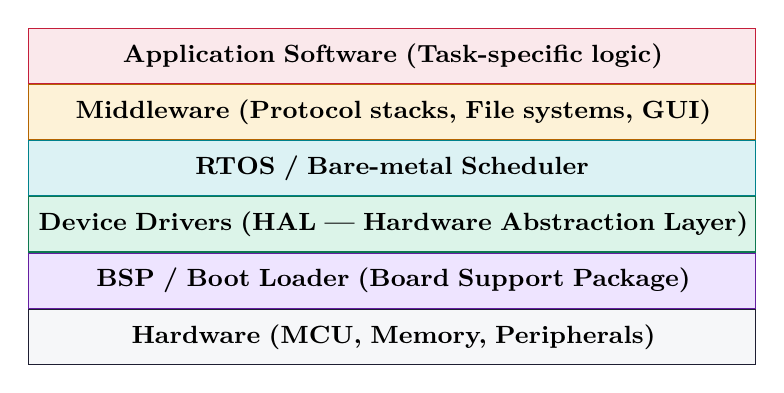
\begin{tikzpicture}[node distance=0.0cm]
  \node[rectangle, draw=myred, fill=hdrred, text width=9cm, align=center,
    minimum height=0.7cm, font=\small\bfseries] (app) {Application Software (Task-specific logic)};
  \node[rectangle, draw=myamber, fill=hdramber, text width=9cm, align=center,
    minimum height=0.7cm, font=\small\bfseries, below=0.0cm of app] (mid) {Middleware (Protocol stacks, File systems, GUI)};
  \node[rectangle, draw=myteal, fill=hdrteal, text width=9cm, align=center,
    minimum height=0.7cm, font=\small\bfseries, below=0.0cm of mid] (rtos) {RTOS / Bare-metal Scheduler};
  \node[rectangle, draw=mygreen, fill=hdrgreen, text width=9cm, align=center,
    minimum height=0.7cm, font=\small\bfseries, below=0.0cm of rtos] (drv) {Device Drivers (HAL --- Hardware Abstraction Layer)};
  \node[rectangle, draw=mypurple, fill=hdrpurple, text width=9cm, align=center,
    minimum height=0.7cm, font=\small\bfseries, below=0.0cm of drv] (bsp) {BSP / Boot Loader (Board Support Package)};
  \node[rectangle, draw=mydark, fill=mygray, text width=9cm, align=center,
    minimum height=0.7cm, font=\small\bfseries, below=0.0cm of bsp] (hw) {Hardware (MCU, Memory, Peripherals)};
\end{tikzpicture}
\end{tcolorbox}

\subsection{Brief Introduction to Embedded Software Categories}
\begin{itemize}[leftmargin=*, itemsep=3pt]
  \item \textbf{Programming Languages Used:} Assembly language (for low-level hardware control), C (most common for embedded), and C++ (for OOP in embedded, limited use).
  \item \textbf{Bare-metal Programming:} No OS; application code runs directly on hardware. Used in simple, resource-constrained systems.
  \item \textbf{RTOS-based Programming:} Uses a real-time OS for multi-task management. Used when multiple functions must run concurrently with timing guarantees.
  \item \textbf{Firmware Updates (OTA):} Modern embedded systems support Over-The-Air updates to patch firmware without physical access.
\end{itemize}

% ===============================================================================
\section{Design Process in Embedded Systems}
% ===============================================================================

The development of an embedded system follows a structured design process to ensure the product meets functional, real-time, power, and cost requirements.

\begin{tcolorbox}[tikzbox, title={Embedded System Design Process Flow}]
\centering
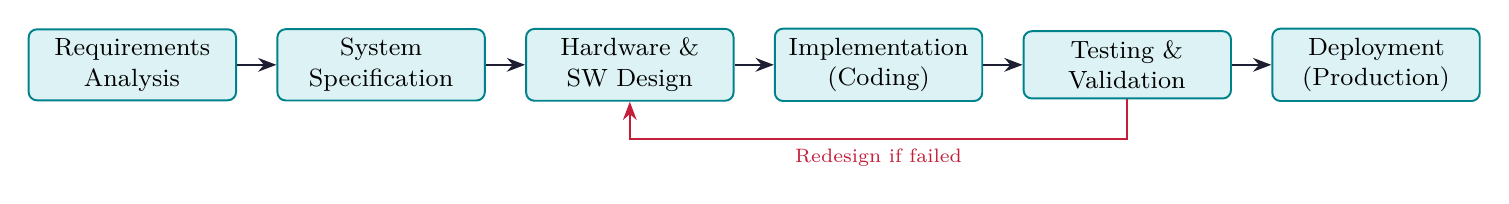
\begin{tikzpicture}[node distance=0.3cm and 0.5cm,
  sblock/.style={rectangle, draw=myteal, fill=hdrteal, text width=2.4cm,
    align=center, minimum height=0.8cm, font=\small, rounded corners=3pt, line width=0.7pt}]
  \node[sblock] (req) {Requirements\\Analysis};
  \node[sblock, right=0.5cm of req] (spec) {System\\Specification};
  \node[sblock, right=0.5cm of spec] (des) {Hardware \&\\SW Design};
  \node[sblock, right=0.5cm of des] (impl) {Implementation\\(Coding)};
  \node[sblock, right=0.5cm of impl] (test) {Testing \&\\Validation};
  \node[sblock, right=0.5cm of test] (dep) {Deployment\\(Production)};

  \draw[arrow] (req) -- (spec);
  \draw[arrow] (spec) -- (des);
  \draw[arrow] (des) -- (impl);
  \draw[arrow] (impl) -- (test);
  \draw[arrow] (test) -- (dep);
  % Feedback arrow
  \draw[redarrow] (test.south) -- ++(0,-0.5) -| (des.south)
    node[pos=0.25, below, font=\scriptsize\color{myred}] {Redesign if failed};
\end{tikzpicture}
\end{tcolorbox}

\subsection{Design Steps Explained}

\begin{enumerate}[label=\textbf{\arabic*.}, leftmargin=*, itemsep=4pt]
  \item \textbf{Requirements Analysis:} Identify what the system must do --- functional requirements (what it does), non-functional requirements (speed, power, cost, size, reliability). Example: ``Control motor speed based on temperature sensor; respond within 10 ms.''
  \item \textbf{System Specification:} Define architecture --- partitioning between hardware and software. Specify processor type, memory size, I/O count, communication protocol, and OS requirements.
  \item \textbf{Hardware Design:} Schematic design (circuit), PCB layout, selection of MCU/processor, memory, power supply IC, and peripheral components.
  \item \textbf{Software Design:} Algorithm design, data flow diagrams, state machines. Choosing programming language (C/Assembly), RTOS selection, ISR design.
  \item \textbf{Implementation:} Writing firmware code (in C or Assembly). Cross-compilation using a host computer to generate binary for the target MCU. Flashing the binary into MCU flash memory.
  \item \textbf{Testing and Validation:} Unit testing (individual modules), integration testing, hardware-in-the-loop (HIL) testing, real-time performance testing. Verify timing deadlines, power consumption, and EMI compliance.
  \item \textbf{Deployment:} Mass production, product integration, final firmware version locked, field testing.
\end{enumerate}

\subsection{Hardware--Software Co-design}

Modern embedded design uses \textbf{hardware--software co-design} --- HW and SW are developed concurrently and their partitioning is optimized to meet cost and performance targets.

\par\noindent
{\renewcommand{\arraystretch}{1.55}%
\begin{tabularx}{\linewidth}{|B{3.2cm}|Y|Y|}
\hline
\textbf{Aspect} & \textbf{Hardware Implementation} & \textbf{Software Implementation} \\
\hline
\textbf{Speed} & Very fast (gate-level logic) & Slower (instruction-by-instruction) \\
\hline
\textbf{Flexibility} & Fixed after fabrication & Easily modified (just reflash) \\
\hline
\textbf{Cost} & High NRE (Non-Recurring Engineering) & Low cost for updates \\
\hline
\textbf{Example} & CRC calculation in FPGA & CRC computed in C function \\
\hline
\end{tabularx}}

% ===============================================================================
% MANDATORY QUICK REVISION PAGE
% ===============================================================================
\newpage
\begin{center}
  {\large\bfseries\color{myred} Quick Revision --- Module 1}\\[3pt]
  {\small\color{mydark} Overview of Embedded Systems $|$ PE-EC703A}
\end{center}
\noindent{\color{myred}\rule{\linewidth}{1.2pt}}
\vspace{4pt}

\begin{tcolorbox}[formulabox, title={\textbf{Key Formulas at a Glance}}]
\renewcommand{\arraystretch}{1.3}
\begin{tabularx}{\linewidth}{B{4.5cm} X}
System Clock Period & $T = \displaystyle\frac{1}{f_{clk}}$ \quad (e.g., 12 MHz clock $\Rightarrow T = 83.3\,\text{ns}$) \\[4pt]
Instruction Cycle & $t_{inst} = \frac{N_{cycles}}{f_{clk}}$ \quad ($N_{cycles}$ = machine cycles per instruction) \\[4pt]
Power Dissipation & $P = C \cdot V_{DD}^2 \cdot f$ \quad (dynamic power in CMOS logic) \\[4pt]
Response Time Deadline & $t_{response} \leq t_{deadline}$ \quad (real-time constraint; must always hold)
\end{tabularx}
\end{tcolorbox}

\begin{tcolorbox}[defbox, title={\textbf{One-Line Definitions}}]
\begin{itemize}[leftmargin=*, itemsep=2.5pt, topsep=0pt]
  \item \textbf{Embedded System:} Dedicated computing system embedded inside a product to perform a specific function with real-time constraints.
  \item \textbf{Firmware:} Software permanently stored in ROM/Flash; directly controls hardware.
  \item \textbf{MCU:} Microcontroller Unit --- CPU, RAM, ROM, and peripherals all on one chip.
  \item \textbf{MPU:} Microprocessor Unit --- CPU only; needs external support chips.
  \item \textbf{RTOS:} Real-Time Operating System --- guarantees task completion within hard time deadlines.
  \item \textbf{HAL:} Hardware Abstraction Layer --- software interface that hides hardware details from application code.
  \item \textbf{BSP:} Board Support Package --- low-level software that initializes specific hardware board peripherals.
  \item \textbf{Bare-metal:} Programming directly on hardware without an operating system.
  \item \textbf{Cross-compiler:} A compiler running on a host PC that generates code for a different target architecture (e.g., ARM).
  \item \textbf{Hard real-time:} System where missing a deadline causes catastrophic failure (e.g., airbag control).
  \item \textbf{Soft real-time:} System where missing a deadline degrades performance but is not fatal (e.g., video streaming).
\end{itemize}
\end{tcolorbox}

\begin{tcolorbox}[exambox, title={\textbf{Frequently Asked / Viva Questions}}]
\begin{enumerate}[topsep=0pt, label=\textbf{Q\arabic*.}, itemsep=5pt]
  \item \Q{Define an embedded system. How does it differ from a general-purpose computer?}
    An embedded system is a dedicated computing unit integrated into a product to perform a specific function (e.g., car ABS controller). A general-purpose computer (PC) can run any program. Embedded systems are resource-constrained, single-function, and often real-time.
  \item \Q{What are the key components of an embedded system?}
    \begin{itemize}[leftmargin=*, itemsep=1pt, topsep=2pt]
      \item Processor (MCU/MPU), Memory (RAM/ROM/Flash), I/O Interfaces
      \item Communication ports (UART, SPI, I2C, CAN), Timers, Clock source, Power supply
    \end{itemize}
  \item \Q{What is the difference between a microprocessor and a microcontroller?}
    A \textbf{microprocessor} contains only the CPU; it needs external RAM, ROM, and peripherals. A \textbf{microcontroller} integrates CPU, RAM, ROM, and peripherals on a single chip --- lower cost, smaller size, less power.
  \item \Q{What is firmware? Where is it stored?}
    Firmware is the embedded software (program code) that directly controls hardware. It is stored in \textbf{non-volatile memory} --- ROM, Flash, or EEPROM --- so it persists after power-off.
  \item \Q{What is meant by real-time in embedded systems?}
    Real-time means the system must complete its tasks within guaranteed time limits (deadlines). In \textbf{hard real-time} systems, missing a deadline causes system failure. In \textbf{soft real-time}, performance degrades but operation continues.
  \item \Q{List the steps in the embedded system design process.}
    Requirements analysis $\to$ System specification $\to$ HW \& SW design $\to$ Implementation (coding) $\to$ Testing and validation $\to$ Deployment.
  \item \Q{What is hardware--software co-design?}
    It is the simultaneous design of hardware and software components, optimizing their partitioning to meet cost, performance, and power goals. Functions can be implemented in either HW (faster, fixed) or SW (flexible, cheaper to modify).
  \item \Q{What is a BSP (Board Support Package)?}
    A BSP is a collection of low-level software routines specific to a hardware board. It initializes the processor, memory, clocks, and peripherals during boot, providing a foundation for higher-level software layers.
  \item \Q{What is a cross-compiler and why is it needed?}
    A cross-compiler runs on a \textbf{host machine} (e.g., x86 PC) and generates executable code for a \textbf{target architecture} (e.g., ARM, 8051). It is needed because embedded targets often lack the resources to run a compiler themselves.
  \item \Q{Give three examples of embedded systems in daily life.}
    Washing machine controller, automobile engine control unit (ECU), digital camera, ATM machine, and smart thermostat.
  \item \Q{What is the role of a bootloader in an embedded system?}
    The bootloader is the first code executed after power-on. It initializes hardware (clocks, memory), and loads the main application firmware from flash into RAM (if needed) and transfers execution control to the application.
  \item \Q{What is meant by a ``resource-constrained'' embedded system?}
    Resource-constrained means the system has very limited RAM (e.g., 256 bytes to 64 KB), flash (8 KB to 1 MB), processing power (8-bit, 8 MHz), and battery capacity. Firmware must be optimized to work within these tight constraints.
\end{enumerate}
\end{tcolorbox}

\begin{tcolorbox}[tikzbox, title={Comparison: Microprocessor vs.\ Microcontroller vs.\ DSP}]
\par\noindent
{\renewcommand{\arraystretch}{1.55}%
\begin{tabularx}{\linewidth}{|B{2.8cm}|Y|Y|Y|}
\hline
\textbf{Feature} & \textbf{Microprocessor} & \textbf{Microcontroller} & \textbf{DSP Processor} \\
\hline
\textbf{Integration} & CPU only & CPU + RAM + ROM + I/O & CPU + MAC unit \\
\hline
\textbf{External Parts} & Many needed & Few or none & Some needed \\
\hline
\textbf{Power} & High & Low & Medium \\
\hline
\textbf{Cost} & High (system level) & Low (single chip) & Medium--High \\
\hline
\textbf{Best For} & Complex OS-based apps & Dedicated control tasks & Signal processing (audio, radar) \\
\hline
\textbf{Example} & Intel Core i7 & PIC16F877, STM32 & TI TMS320C6748 \\
\hline
\end{tabularx}}
\end{tcolorbox}


% -- Module 2 -----------------------------------------------------------------
\modulestart{2}{8051 Microcontroller --- Architecture Overview}

\section{8051 Microcontroller --- Architecture Overview}
% ===============================================================================

The Intel 8051 is an 8-bit microcontroller introduced in 1980. It is one of the most widely taught architectures in embedded systems education due to its simplicity and self-contained design.

\begin{tcolorbox}[defbox, title={\textbf{8051 Microcontroller}}]
The \textbf{8051} is an 8-bit, single-chip microcontroller with on-chip program memory (ROM), data memory (RAM), I/O ports, timers, a serial port, and interrupt logic. It operates on a Harvard architecture (separate program and data memory buses).
\end{tcolorbox}

\subsection{Key Features of 8051}
\begin{itemize}[leftmargin=*, itemsep=3pt]
  \item \textbf{CPU:} 8-bit ALU, accumulator (A), B register, PSW (Program Status Word).
  \item \textbf{ROM (Program Memory):} 4 KB on-chip; expandable to 64 KB externally.
  \item \textbf{RAM (Data Memory):} 128 bytes on-chip; upper 128 bytes are SFRs (Special Function Registers).
  \item \textbf{I/O Ports:} Four 8-bit bidirectional I/O ports (P0, P1, P2, P3).
  \item \textbf{Timers:} Two 16-bit timers/counters (Timer 0 and Timer 1).
  \item \textbf{Serial Port (UART):} Full-duplex serial communication (TXD/RXD on P3).
  \item \textbf{Interrupts:} Five interrupt sources --- INT0, INT1, Timer0, Timer1, Serial.
  \item \textbf{Clock:} Typically 12 MHz crystal; one machine cycle = 12 clock cycles.
\end{itemize}

\begin{tcolorbox}[tikzbox, title={8051 Internal Architecture Block Diagram}]
\centering
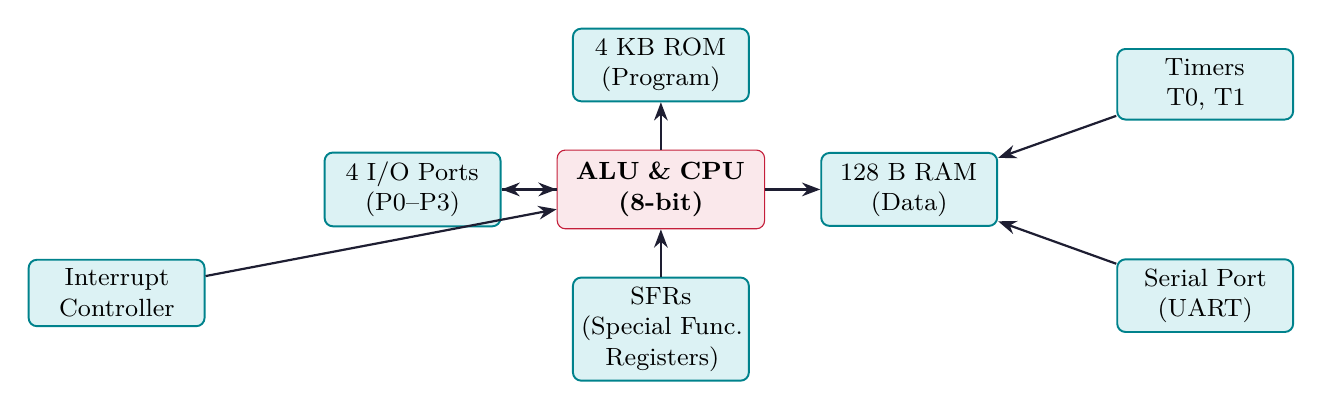
\begin{tikzpicture}[node distance=0.3cm and 0.5cm,
  sblock/.style={rectangle, draw=myteal, fill=hdrteal, text width=2.0cm,
    align=center, minimum height=0.8cm, font=\small, rounded corners=3pt, line width=0.7pt}]
  \node[rectangle, draw=myred, fill=hdrred, text width=2.4cm, align=center,
    minimum height=1.0cm, font=\small\bfseries, rounded corners=3pt] (alu) {ALU \& CPU\\(8-bit)};
  \node[sblock, above=0.6cm of alu] (rom) {4 KB ROM\\(Program)};
  \node[sblock, right=0.7cm of alu] (ram) {128 B RAM\\(Data)};
  \node[sblock, below=0.6cm of alu] (sfr) {SFRs\\(Special Func.\\Registers)};
  \node[sblock, left=0.7cm of alu] (io) {4 I/O Ports\\(P0--P3)};
  \node[sblock, above right=0.4cm and 1.5cm of ram] (tmr) {Timers\\T0, T1};
  \node[sblock, below right=0.4cm and 1.5cm of ram] (ser) {Serial Port\\(UART)};
  \node[sblock, below left=0.4cm and 1.5cm of io] (intr) {Interrupt\\Controller};

  \draw[arrow] (alu) -- (rom);
  \draw[arrow] (alu) -- (ram);
  \draw[arrow] (sfr) -- (alu);
  \draw[arrow] (io) -- (alu);
  \draw[arrow] (alu) -- (io);
  \draw[arrow] (tmr) -- (ram);
  \draw[arrow] (ser) -- (ram);
  \draw[arrow] (intr) -- (alu);
\end{tikzpicture}
\end{tcolorbox}

\subsection{Real-World Interfacing of 8051}
\begin{itemize}[leftmargin=*, itemsep=3pt]
  \item \textbf{LED / Switch:} GPIO pins directly drive LEDs (with current-limiting resistors); switches pulled up to VCC.
  \item \textbf{LCD (16x2):} Driven via P2 (data bus) and P3 control lines (RS, RW, EN).
  \item \textbf{ADC (e.g., ADC0804):} External ADC connected via parallel data bus and control signals.
  \item \textbf{Stepper Motor:} Driven via ULN2003 driver IC connected to P1.
  \item \textbf{Serial Communication:} TXD (P3.1) and RXD (P3.0) connect to MAX232 (RS-232 level converter) for PC communication.
\end{itemize}

% ===============================================================================
\section{ARM Processor Architecture}
% ===============================================================================

\begin{tcolorbox}[defbox, title={\textbf{ARM (Advanced RISC Machine) Processor}}]
\textbf{ARM} is a family of RISC (Reduced Instruction Set Computer) processor architectures developed by ARM Holdings. ARM processors are characterized by a 32-bit (or 64-bit) load-store architecture, fixed-length 32-bit instructions (Thumb: 16-bit compressed), low power consumption, and high code density.
\end{tcolorbox}

\subsection{ARM vs.\ 8051 --- Key Differences}

\par\noindent
{\renewcommand{\arraystretch}{1.6}%
\begin{tabularx}{\linewidth}{|B{3.0cm}|Y|Y|}
\hline
\textbf{Feature} & \textbf{8051} & \textbf{ARM Cortex-M} \\
\hline
\textbf{Architecture} & CISC (8-bit, Harvard) & RISC (32-bit, Harvard) \\
\hline
\textbf{Registers} & A, B, R0--R7 (bank-switched) & 16 general-purpose 32-bit registers (R0--R15) \\
\hline
\textbf{Clock Speed} & 12 MHz (typical) & Up to 168 MHz+ (Cortex-M4) \\
\hline
\textbf{Pipeline} & Single-stage & 3-stage (Cortex-M0) to 6-stage (Cortex-M4) \\
\hline
\textbf{Instruction Set} & Complex, variable-length & RISC + Thumb-2 (16/32-bit) \\
\hline
\textbf{Built-in DSP} & No & Yes (Cortex-M4 has FPU + DSP extensions) \\
\hline
\textbf{Power} & Low (simple core) & Ultra-low to medium \\
\hline
\textbf{Example Chips} & AT89S52, DS89C4x0 & STM32, LPC1768, Nordic nRF52 \\
\hline
\end{tabularx}}

\subsection{ARM Processor Features}
\begin{itemize}[leftmargin=*, itemsep=3pt]
  \item \textbf{RISC Pipeline:} Multi-stage instruction pipeline (Fetch $\to$ Decode $\to$ Execute) allows higher throughput.
  \item \textbf{Load-Store Architecture:} Only Load and Store instructions access memory; all other operations work on registers.
  \item \textbf{Thumb Instruction Set:} 16-bit compressed instructions reduce code size by $\sim$30\% while maintaining most of the 32-bit performance.
  \item \textbf{Barrel Shifter:} Integrated into ALU --- allows free-of-cost shifts/rotates within any data-processing instruction.
  \item \textbf{NVIC (Nested Vectored Interrupt Controller):} Fast, low-latency interrupt handling with configurable priority levels.
  \item \textbf{Cortex-M Variants:} M0 (ultra-low power), M3 (general purpose), M4 (with FPU and DSP), M7 (high performance).
\end{itemize}

% ===============================================================================
\section{Processor and Memory Organization}
% ===============================================================================

\subsection{Memory Types in Embedded Systems}

\par\noindent
{\renewcommand{\arraystretch}{1.6}%
\begin{tabularx}{\linewidth}{|B{3.0cm}|Y|Y|}
\hline
\textbf{Memory Type} & \textbf{Characteristics} & \textbf{Use in Embedded} \\
\hline
\textbf{ROM} (Mask ROM) & Non-volatile, factory-programmed, read-only & Fixed firmware in mass-produced ICs \\
\hline
\textbf{Flash} & Non-volatile, electrically erasable, page-by-page write & Main program storage in modern MCUs \\
\hline
\textbf{EEPROM} & Non-volatile, byte-wise electrically erasable & Configuration data, calibration parameters \\
\hline
\textbf{SRAM} & Volatile, fast, no refresh needed & CPU data memory, stack, heap \\
\hline
\textbf{DRAM} & Volatile, needs refresh, high density & External memory for complex embedded systems (not MCU) \\
\hline
\textbf{SDRAM} & Synchronous DRAM, higher speed & External RAM for embedded Linux (e.g., Raspberry Pi) \\
\hline
\end{tabularx}}

\subsection{Harvard vs.\ Von Neumann Architecture}

\par\noindent
{\renewcommand{\arraystretch}{1.55}%
\begin{tabularx}{\linewidth}{|B{3.0cm}|Y|Y|}
\hline
\textbf{Feature} & \textbf{Harvard Architecture} & \textbf{Von Neumann Architecture} \\
\hline
\textbf{Memory Buses} & Separate instruction and data buses & Single shared bus \\
\hline
\textbf{Simultaneous Access} & Yes --- fetch instruction while reading data & No --- only one at a time \\
\hline
\textbf{Speed} & Faster (no bus contention) & Slower (bus bottleneck) \\
\hline
\textbf{Examples} & 8051, PIC, ARM Cortex-M & Intel x86 PC \\
\hline
\textbf{Complexity} & Higher (dual bus hardware) & Simpler \\
\hline
\end{tabularx}}

\subsection{Memory Map of a Typical MCU}

The memory-mapped addressing scheme of a microcontroller assigns fixed addresses to each memory region:

\begin{tcolorbox}[tikzbox, title={Typical MCU Memory Map (ARM Cortex-M)}]
\centering
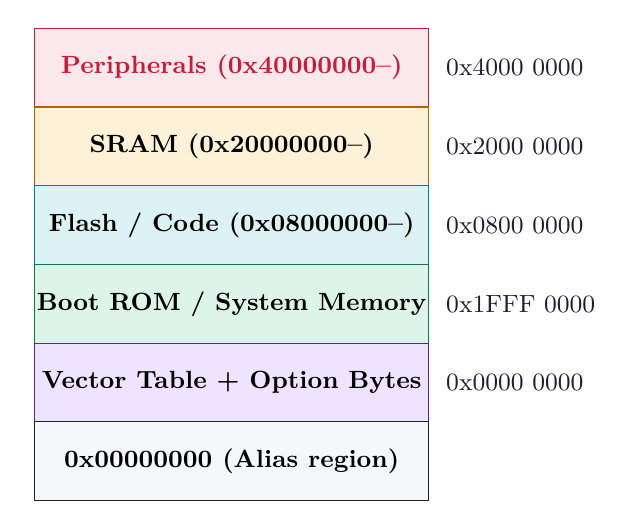
\begin{tikzpicture}[scale=1.0, every node/.style={font=\small}]
  % Memory blocks stacked vertically
  \draw[fill=hdrred, draw=myred] (0,5.0) rectangle (5,6.0)
    node[midway, font=\small\bfseries, color=myred] {Peripherals (0x40000000--)};
  \draw[fill=hdramber, draw=myamber] (0,4.0) rectangle (5,5.0)
    node[midway, font=\small\bfseries] {SRAM (0x20000000--)};
  \draw[fill=hdrteal, draw=myteal] (0,3.0) rectangle (5,4.0)
    node[midway, font=\small\bfseries] {Flash / Code (0x08000000--)};
  \draw[fill=hdrgreen, draw=mygreen] (0,2.0) rectangle (5,3.0)
    node[midway, font=\small\bfseries] {Boot ROM / System Memory};
  \draw[fill=hdrpurple, draw=mypurple] (0,1.0) rectangle (5,2.0)
    node[midway, font=\small\bfseries] {Vector Table + Option Bytes};
  \draw[fill=mygray, draw=mydark] (0,0.0) rectangle (5,1.0)
    node[midway, font=\small\bfseries] {0x00000000 (Alias region)};
  % Addresses
  \node[right, color=mydark] at (5.1, 5.5) {0x4000 0000};
  \node[right, color=mydark] at (5.1, 4.5) {0x2000 0000};
  \node[right, color=mydark] at (5.1, 3.5) {0x0800 0000};
  \node[right, color=mydark] at (5.1, 2.5) {0x1FFF 0000};
  \node[right, color=mydark] at (5.1, 1.5) {0x0000 0000};
\end{tikzpicture}
\end{tcolorbox}

% ===============================================================================
\section{Parallelism in Instruction Level}
% ===============================================================================

\begin{tcolorbox}[defbox, title={\textbf{Instruction-Level Parallelism (ILP)}}]
\textbf{Instruction-Level Parallelism (ILP)} is the ability of a processor to execute multiple instructions simultaneously, overlapping their execution stages using techniques such as \textbf{pipelining}, \textbf{superscalar execution}, and \textbf{VLIW} (Very Long Instruction Word).
\end{tcolorbox}

\subsection{Pipelining}

Pipelining divides instruction execution into \textbf{stages}, so that multiple instructions can be in different stages of execution simultaneously --- like an assembly line.

\begin{tcolorbox}[tikzbox, title={3-Stage Instruction Pipeline (ARM Cortex-M0)}]
\centering
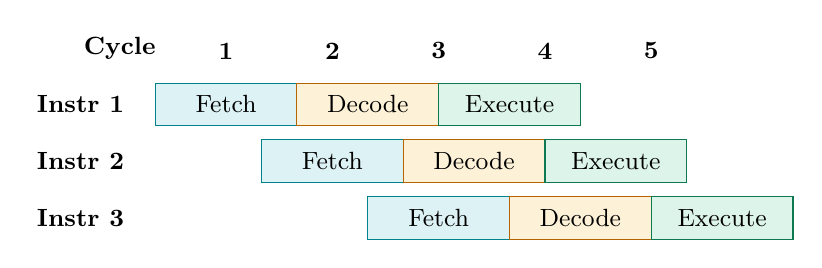
\begin{tikzpicture}[scale=0.9, every node/.style={font=\small}]
  % Stage labels
  \node[above] at (1.0, 3.2) {\textbf{Cycle}};
  \node[above] at (2.5, 3.2) {\textbf{1}};
  \node[above] at (4.0, 3.2) {\textbf{2}};
  \node[above] at (5.5, 3.2) {\textbf{3}};
  \node[above] at (7.0, 3.2) {\textbf{4}};
  \node[above] at (8.5, 3.2) {\textbf{5}};

  % Instruction 1
  \node[left] at (1.2, 2.7) {\textbf{Instr 1}};
  \draw[fill=hdrteal, draw=myteal] (1.5,2.4) rectangle (3.5,3.0) node[midway] {Fetch};
  \draw[fill=hdramber, draw=myamber] (3.5,2.4) rectangle (5.5,3.0) node[midway] {Decode};
  \draw[fill=hdrgreen, draw=mygreen] (5.5,2.4) rectangle (7.5,3.0) node[midway] {Execute};

  % Instruction 2
  \node[left] at (1.2, 1.9) {\textbf{Instr 2}};
  \draw[fill=hdrteal, draw=myteal] (3.0,1.6) rectangle (5.0,2.2) node[midway] {Fetch};
  \draw[fill=hdramber, draw=myamber] (5.0,1.6) rectangle (7.0,2.2) node[midway] {Decode};
  \draw[fill=hdrgreen, draw=mygreen] (7.0,1.6) rectangle (9.0,2.2) node[midway] {Execute};

  % Instruction 3
  \node[left] at (1.2, 1.1) {\textbf{Instr 3}};
  \draw[fill=hdrteal, draw=myteal] (4.5,0.8) rectangle (6.5,1.4) node[midway] {Fetch};
  \draw[fill=hdramber, draw=myamber] (6.5,0.8) rectangle (8.5,1.4) node[midway] {Decode};
  \draw[fill=hdrgreen, draw=mygreen] (8.5,0.8) rectangle (10.5,1.4) node[midway] {Execute};
\end{tikzpicture}
\end{tcolorbox}

\subsection{Pipeline Hazards}

\par\noindent
{\renewcommand{\arraystretch}{1.55}%
\begin{tabularx}{\linewidth}{|B{3.0cm}|Y|Y|}
\hline
\textbf{Hazard Type} & \textbf{Cause} & \textbf{Solution} \\
\hline
\textbf{Data Hazard} & Instruction depends on result of a previous instruction still in pipeline & Register forwarding (bypassing), stall/bubble insertion \\
\hline
\textbf{Control Hazard} & Branch instruction changes program flow before pipeline completes & Branch prediction, pipeline flush \\
\hline
\textbf{Structural Hazard} & Two instructions need same hardware resource simultaneously & Resource duplication, stall \\
\hline
\end{tabularx}}

% ===============================================================================
\section{Processor and Memory Selection}
% ===============================================================================

Selecting the right processor and memory for an embedded application requires balancing multiple constraints:

\begin{tcolorbox}[formulabox, title={\textbf{Processor Selection Criteria}}]
\begin{itemize}[leftmargin=*, itemsep=3pt]
  \item \textbf{Processing Speed:} Clock frequency (MHz) and MIPS (Million Instructions Per Second) rating.
  \item \textbf{Word Width:} 8-bit (simple, low-cost) vs.\ 16-bit vs.\ 32-bit (high performance).
  \item \textbf{On-chip Peripherals:} Required ADC channels, communication ports, timers.
  \item \textbf{Power Consumption:} Active current ($I_{DD}$), sleep current ($I_{standby}$) --- critical for battery-powered devices.
  \item \textbf{Cost:} Unit price must fit product BOM (Bill of Materials) budget.
  \item \textbf{Toolchain and Ecosystem:} Availability of compilers, debuggers, libraries, and community support.
  \item \textbf{Temperature Range:} Industrial ($-40^{\circ}$C to $+85^{\circ}$C), automotive ($-40^{\circ}$C to $+125^{\circ}$C).
\end{itemize}
\end{tcolorbox}

\subsection{Memory Selection Criteria}
\begin{itemize}[leftmargin=*, itemsep=3pt]
  \item \textbf{Volatile vs.\ Non-volatile:} Program code needs non-volatile (Flash); variables need volatile (SRAM).
  \item \textbf{Capacity:} Must accommodate program code, constants, variables, stack, and heap with margin.
  \item \textbf{Access Speed:} RAM access time must be compatible with processor clock (no wait states needed).
  \item \textbf{Endurance:} Flash has limited write cycles ($\sim$100,000 erase/write cycles) --- critical for OTA update designs.
  \item \textbf{Interface:} Parallel bus (faster) vs.\ serial (SPI/I2C Flash --- slower but fewer pins).
\end{itemize}

% ===============================================================================
% MANDATORY QUICK REVISION PAGE
% ===============================================================================
\newpage
\begin{center}
  {\large\bfseries\color{myred} Quick Revision --- Module 2}\\[3pt]
  {\small\color{mydark} Embedded Hardware: Processor \& Memory $|$ PE-EC703A}
\end{center}
\noindent{\color{myred}\rule{\linewidth}{1.2pt}}
\vspace{4pt}

\begin{tcolorbox}[formulabox, title={\textbf{Key Formulas at a Glance}}]
\renewcommand{\arraystretch}{1.3}
\begin{tabularx}{\linewidth}{B{4.5cm} X}
Machine Cycle Time (8051) & $t_{mc} = \displaystyle\frac{12}{f_{osc}}$ \quad (12 oscillator periods per machine cycle) \\[4pt]
Processing Speed & $\text{MIPS} = \displaystyle\frac{f_{clk}}{CPI \times 10^6}$ \quad (CPI = Cycles Per Instruction) \\[4pt]
Pipeline Speedup & $S = \displaystyle\frac{t_{no\text{-}pipeline}}{t_{pipeline}} \approx N$ \quad ($N$ = number of stages, ideal) \\[4pt]
Memory Address Space & $\text{Addressable locations} = 2^n$ \quad ($n$ = address bus width in bits)
\end{tabularx}
\end{tcolorbox}

\begin{tcolorbox}[defbox, title={\textbf{One-Line Definitions}}]
\begin{itemize}[leftmargin=*, itemsep=2.5pt, topsep=0pt]
  \item \textbf{8051:} An 8-bit Harvard-architecture microcontroller with 4 KB ROM, 128 B RAM, 4 I/O ports, and 2 timers.
  \item \textbf{ARM:} Advanced RISC Machine; 32-bit low-power RISC processor widely used in embedded and mobile devices.
  \item \textbf{RISC:} Reduced Instruction Set Computer --- few, simple, fixed-length instructions; high clock rate.
  \item \textbf{Harvard Architecture:} Separate buses for program memory and data memory allowing simultaneous access.
  \item \textbf{Von Neumann:} Single shared bus for instructions and data; simpler but slower.
  \item \textbf{Pipeline:} Technique to overlap execution of multiple instructions by dividing into fetch-decode-execute stages.
  \item \textbf{ILP:} Instruction-Level Parallelism --- executing multiple instructions in the same clock cycle.
  \item \textbf{Flash Memory:} Non-volatile, electrically erasable memory used to store program code in MCUs.
  \item \textbf{SRAM:} Static RAM --- volatile, fast, no refresh; used for data memory and stack in MCUs.
  \item \textbf{SFR:} Special Function Register in 8051 (addresses 80H--FFH) controlling timers, serial port, I/O, interrupts.
  \item \textbf{Thumb Instruction Set:} 16-bit compressed ARM instruction set reducing code size by $\sim$30\%.
  \item \textbf{NVIC:} Nested Vectored Interrupt Controller in ARM; handles priority-based, low-latency interrupts.
\end{itemize}
\end{tcolorbox}

\begin{tcolorbox}[exambox, title={\textbf{Frequently Asked / Viva Questions}}]
\begin{enumerate}[topsep=0pt, label=\textbf{Q\arabic*.}, itemsep=5pt]
  \item \Q{What is the architecture of the 8051 microcontroller?}
    The 8051 is an 8-bit Harvard-architecture MCU with a 4 KB ROM (program), 128 bytes RAM (data), four 8-bit I/O ports, two 16-bit timers, one UART serial port, and five interrupt sources. One machine cycle = 12 oscillator clock cycles.
  \item \Q{What is the difference between Harvard and Von Neumann architecture?}
    Harvard uses separate buses for program and data memory, enabling simultaneous fetch and data access (faster). Von Neumann uses a single bus for both (simpler but has bottleneck). 8051 and ARM MCUs use Harvard; x86 PCs use Von Neumann.
  \item \Q{What is pipelining? What is its advantage?}
    Pipelining divides instruction execution into stages (Fetch, Decode, Execute) and processes multiple instructions concurrently in different stages. Advantage: Increases throughput (instructions completed per clock cycle) without increasing clock frequency.
  \item \Q{Name the three types of pipeline hazards.}
    \begin{itemize}[leftmargin=*, itemsep=1pt, topsep=2pt]
      \item \textbf{Data Hazard:} Dependency between instructions (solved by forwarding/stall).
      \item \textbf{Control Hazard:} Branch instructions disrupting pipeline flow (solved by branch prediction).
      \item \textbf{Structural Hazard:} Two instructions compete for same hardware resource.
    \end{itemize}
  \item \Q{Why is ARM preferred over 8051 for modern embedded systems?}
    ARM (Cortex-M) offers 32-bit data width, higher clock speeds (up to 168 MHz), a pipelined RISC core, Thumb instruction set for code efficiency, built-in NVIC, optional FPU/DSP, and ultra-low power modes. 8051 is only 8-bit and runs at 12 MHz.
  \item \Q{What is the Thumb instruction set in ARM?}
    Thumb is a 16-bit compressed version of the 32-bit ARM instruction set. It reduces code size by $\sim$30\% while retaining most of the performance, making it ideal for memory-constrained embedded systems.
  \item \Q{What are Special Function Registers (SFRs) in 8051?}
    SFRs are memory-mapped registers (addresses 80H--FFH) that control the MCU's internal peripherals such as ports (P0--P3), timers (TCON, TMOD), serial port (SCON, SBUF), interrupt control (IE, IP), and the stack pointer (SP).
  \item \Q{What is the difference between Flash memory and EEPROM?}
    Flash memory is erased in large \textbf{blocks/pages} and is much faster and higher-density --- used for program code storage. EEPROM is erased byte-by-byte (or word-by-word), has fewer erase cycles, but allows fine-grained updates --- used for configuration data.
  \item \Q{What factors are considered in processor selection for an embedded system?}
    Processing speed (MIPS), word width (8/16/32-bit), on-chip peripheral set, power consumption, operating temperature range, unit cost, and availability of compilers, development tools, and community support.
  \item \Q{What is memory-mapped I/O?}
    In memory-mapped I/O, peripheral registers (I/O ports, timers, UART) are assigned addresses in the same address space as RAM. The processor accesses them using regular memory read/write instructions --- no separate I/O instructions needed (used in ARM Cortex-M).
  \item \Q{What is the significance of the barrel shifter in ARM?}
    The barrel shifter in ARM's ALU allows any data-processing instruction to optionally shift or rotate one of its source operands by any amount \textbf{in the same clock cycle} as the main operation --- effectively providing free shift operations.
  \item \Q{What is MIPS and how is it calculated?}
    MIPS (Million Instructions Per Second) measures processor performance. $\text{MIPS} = f_{clk} / (CPI \times 10^6)$ where CPI is Cycles Per Instruction. For 8051 at 12 MHz with CPI = 12: MIPS $= 12/(12) = 1$ MIPS.
\end{enumerate}
\end{tcolorbox}

\begin{tcolorbox}[tikzbox, title={8051 vs.\ ARM Cortex-M --- At a Glance}]
\par\noindent
{\renewcommand{\arraystretch}{1.55}%
\begin{tabularx}{\linewidth}{|B{2.8cm}|Y|Y|}
\hline
\textbf{Parameter} & \textbf{8051} & \textbf{ARM Cortex-M4} \\
\hline
\textbf{Data Width} & 8-bit & 32-bit \\
\hline
\textbf{Max Clock} & 12 MHz (standard) & 168 MHz \\
\hline
\textbf{Architecture} & Harvard, CISC-like & Harvard, RISC \\
\hline
\textbf{Pipeline} & None & 6-stage \\
\hline
\textbf{On-chip Flash} & 4 KB (original) & Up to 2 MB \\
\hline
\textbf{On-chip SRAM} & 128 bytes & Up to 256 KB \\
\hline
\textbf{FPU} & No & Yes (single precision) \\
\hline
\textbf{Interrupts} & 5 sources & Up to 240 (NVIC) \\
\hline
\end{tabularx}}
\end{tcolorbox}


% -- Module 3 -----------------------------------------------------------------
\modulestart{3}{Serial and Parallel Communication Ports}

\section{Serial and Parallel Communication Ports}
% ===============================================================================

\begin{tcolorbox}[defbox, title={\textbf{Serial vs.\ Parallel Communication}}]
\textbf{Serial Communication:} Data is transmitted one bit at a time over a single wire (or differential pair). Slower per line but uses fewer wires, suitable for long-distance communication.

\textbf{Parallel Communication:} Multiple bits (e.g., 8 bits) are transmitted simultaneously over multiple wires. Faster but requires more wires; limited to short distances due to skew and crosstalk.
\end{tcolorbox}

\par\noindent
{\renewcommand{\arraystretch}{1.55}%
\begin{tabularx}{\linewidth}{|B{3.0cm}|Y|Y|}
\hline
\textbf{Feature} & \textbf{Serial Port (UART)} & \textbf{Parallel Port} \\
\hline
\textbf{Wires} & 2 (TXD, RXD) minimum & 8+ data lines + control \\
\hline
\textbf{Speed} & Lower (per port) & Higher \\
\hline
\textbf{Distance} & Long range (RS-232, RS-485) & Short (PCB-level, $<$1 m) \\
\hline
\textbf{Cost} & Low (fewer pins, simpler hardware) & Higher \\
\hline
\textbf{Examples} & UART, SPI, I2C, USB & 8051 P0--P3 ports, old printer port \\
\hline
\end{tabularx}}

\subsection{UART (Universal Asynchronous Receiver/Transmitter)}
\begin{itemize}[leftmargin=*, itemsep=3pt]
  \item \textbf{Asynchronous:} No shared clock line --- both devices agree on \textbf{baud rate} beforehand.
  \item \textbf{Frame format:} Start bit (1, low) + Data bits (5--9) + Optional Parity bit + Stop bit(s) (1 or 2, high).
  \item \textbf{Baud rate:} Number of signal changes per second (symbols/second). At 9600 baud, 1 bit = 104 $\mu$s.
  \item \textbf{Wiring:} TXD of device A connects to RXD of device B, and vice versa. Ground is shared.
\end{itemize}

\begin{tcolorbox}[formulabox, title={\textbf{UART Baud Rate Formula (8051)}}]
\[
\text{Baud Rate} = \frac{f_{osc}}{32 \times 12 \times (256 - \text{TH1})}
\quad \text{(Mode 1 or 3, Timer 1 in 8-bit auto-reload)}
\]
For 9600 baud at $f_{osc} = 11.0592\,\text{MHz}$: \quad TH1 = FDH (253)
\end{tcolorbox}

% ===============================================================================
\section{Timer and Counting Devices}
% ===============================================================================

\begin{tcolorbox}[defbox, title={\textbf{Timer / Counter}}]
A \textbf{timer} is a hardware counter that increments on each internal clock pulse (counting time). A \textbf{counter} increments on each external event pulse (e.g., counting RPM or pulses). Both use the same hardware register; the source of the clock selects timer vs.\ counter mode.
\end{tcolorbox}

\subsection{8051 Timer Modes}

The 8051 has two timers (Timer 0 and Timer 1), each configurable in 4 modes via TMOD register:

\par\noindent
{\renewcommand{\arraystretch}{1.55}%
\begin{tabularx}{\linewidth}{|B{2.5cm}|Y|Y|}
\hline
\textbf{Mode} & \textbf{Description} & \textbf{Use} \\
\hline
\textbf{Mode 0} & 13-bit timer/counter (TH + 5 LSBs of TL) & Legacy 8048 compatibility \\
\hline
\textbf{Mode 1} & 16-bit timer/counter (TH:TL = 65536 counts) & Long time delays \\
\hline
\textbf{Mode 2} & 8-bit auto-reload (TL counts, TH is reload value) & Baud rate generation \\
\hline
\textbf{Mode 3} & Two independent 8-bit timers (Timer 0 only) & Dual-purpose timing \\
\hline
\end{tabularx}}

\begin{tcolorbox}[formulabox, title={\textbf{Timer Delay Calculation (8051, Mode 1)}}]
\[
\text{Time delay} = (65536 - \text{Initial Count}) \times \frac{12}{f_{osc}}
\]
Example: For 10 ms delay at 12 MHz: Initial Count $= 65536 - 10000 = 55536 =$ D8F0H
\end{tcolorbox}

% ===============================================================================
\section{Watchdog Timer}
% ===============================================================================

\begin{tcolorbox}[defbox, title={\textbf{Watchdog Timer (WDT)}}]
A \textbf{watchdog timer} is a hardware timer that automatically \textbf{resets the microcontroller} if the software fails to periodically reset (``kick'' or ``pet'') it within a defined time interval. It is used to detect and recover from software deadlocks, infinite loops, or crashes in embedded systems.
\end{tcolorbox}

\subsection{Watchdog Timer Operation}

\begin{tcolorbox}[tikzbox, title={Watchdog Timer Operation Flow}]
\centering
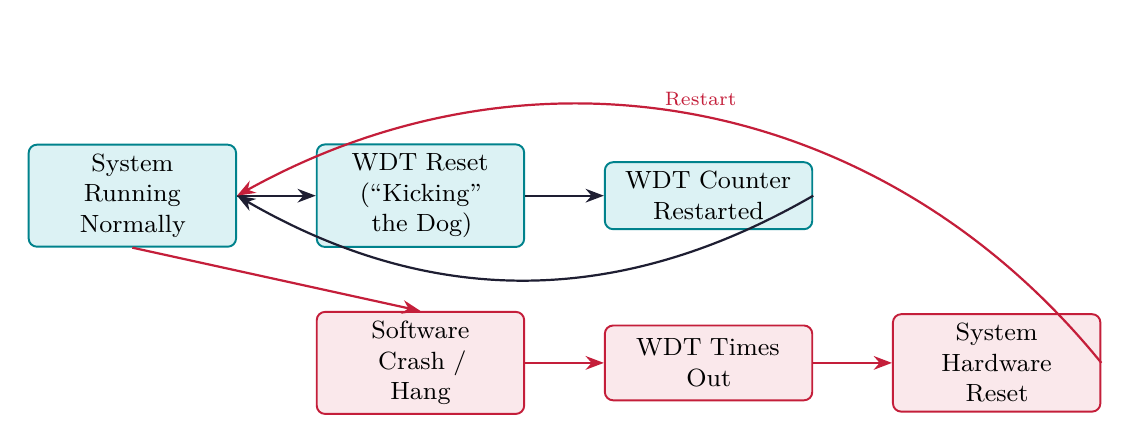
\begin{tikzpicture}[node distance=0.5cm and 1.2cm,
  sblock/.style={rectangle, draw=myteal, fill=hdrteal, text width=2.4cm,
    align=center, minimum height=0.8cm, font=\small, rounded corners=3pt, line width=0.7pt}]
  \node[sblock] (run) {System\\Running\\Normally};
  \node[sblock, right=1.0cm of run] (kick) {WDT Reset\\(``Kicking''\\the Dog)};
  \node[sblock, right=1.0cm of kick] (cnt) {WDT Counter\\Restarted};
  \node[redblock, below=0.8cm of kick] (crash) {Software\\Crash /\\Hang};
  \node[redblock, right=1.0cm of crash] (timeout) {WDT Times\\Out};
  \node[redblock, right=1.0cm of timeout] (reset) {System\\Hardware\\Reset};

  \draw[arrow] (run) -- (kick);
  \draw[arrow] (kick) -- (cnt);
  \draw[arrow] (cnt.east) to[bend left=30] (run.east);
  \draw[redarrow] (run.south) -- (crash.north);
  \draw[redarrow] (crash) -- (timeout);
  \draw[redarrow] (timeout) -- (reset);
  \draw[redarrow] (reset.east) to[bend right=40] node[above, font=\scriptsize\color{myred}] {Restart} (run.east);
\end{tikzpicture}
\end{tcolorbox}

\begin{itemize}[leftmargin=*, itemsep=3pt]
  \item \textbf{Kicking (petting) the WDT:} Software writes a specific value to the WDT register before the timeout period expires. This restarts the countdown.
  \item \textbf{WDT Timeout Period:} Configurable (e.g., 100 ms to several seconds). If not reset in this time, the WDT asserts a hardware reset signal.
  \item \textbf{Window Watchdog (WWDT):} Advanced variant --- must be kicked \textit{within} a specific time window (not too early, not too late) to detect stuck loops that still kick the WDT.
\end{itemize}

% ===============================================================================
\section{Real-Time Clock (RTC)}
% ===============================================================================

\begin{tcolorbox}[defbox, title={\textbf{Real-Time Clock (RTC)}}]
An \textbf{RTC} is a dedicated counter/timer circuit that tracks the current time (hours, minutes, seconds) and date (day, month, year) continuously --- even when the main system is powered off --- using a separate battery (e.g., CR2032 coin cell) and a 32.768 kHz crystal.
\end{tcolorbox}

\begin{itemize}[leftmargin=*, itemsep=3pt]
  \item \textbf{Crystal Frequency:} 32.768 kHz = $2^{15}$ Hz. A 15-bit counter overflows exactly once per second.
  \item \textbf{Interface:} Typically I2C or SPI serial interface (e.g., DS3231, PCF8563).
  \item \textbf{Applications:} Data loggers, digital clocks, alarm systems, access control systems.
  \item \textbf{Alarms/Interrupts:} RTC can generate periodic interrupts (every second, minute, etc.) to wake up the MCU from sleep mode.
\end{itemize}

% ===============================================================================
\section{Serial Bus Communication Protocols}
% ===============================================================================

\subsection{I2C (Inter-Integrated Circuit) Protocol}

\begin{tcolorbox}[defbox, title={\textbf{I2C Protocol}}]
\textbf{I2C} (pronounced ``I-squared-C'') is a synchronous, multi-master, multi-slave, half-duplex serial protocol using only \textbf{two wires}: SDA (Serial Data) and SCL (Serial Clock). Developed by Philips (NXP). Each device has a unique 7-bit (or 10-bit) address.
\end{tcolorbox}

\begin{itemize}[leftmargin=*, itemsep=3pt]
  \item \textbf{Wires:} SDA (bidirectional data) + SCL (clock generated by master). Both are open-drain with pull-up resistors.
  \item \textbf{Speed Modes:} Standard (100 kbps), Fast (400 kbps), Fast-Plus (1 Mbps), High-Speed (3.4 Mbps).
  \item \textbf{Start/Stop Condition:} Start = SDA falls while SCL is high. Stop = SDA rises while SCL is high.
  \item \textbf{ACK/NACK:} After each 8-bit byte, receiver pulls SDA low (ACK) or leaves it high (NACK).
  \item \textbf{Applications:} Connecting sensors (temperature, pressure), EEPROMs, RTC modules, LCD controllers.
\end{itemize}

\begin{tcolorbox}[tikzbox, title={I2C Bus --- Master--Slave Connection}]
\centering
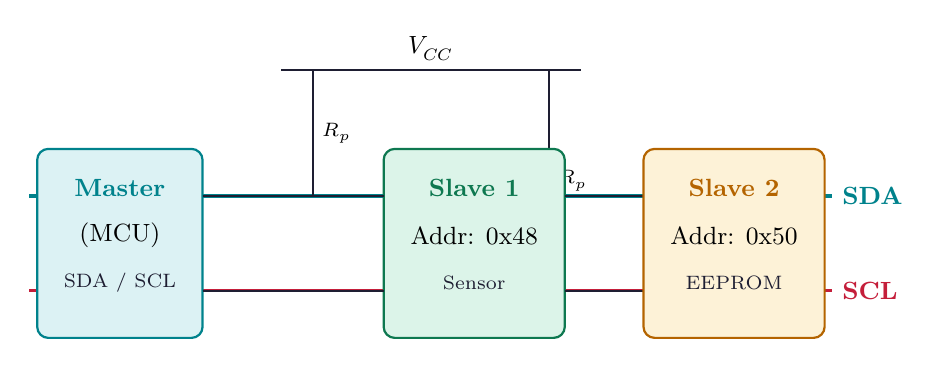
\begin{tikzpicture}[every node/.style={font=\small}, x=1cm, y=1cm]
  % ── Bus lines ──────────────────────────────────────────────────────
  \draw[color=myteal, line width=1.2pt] (0, 2.0) -- (10.2, 2.0);  % SDA
  \draw[color=myred,  line width=1.2pt] (0, 0.8) -- (10.2, 0.8);  % SCL
  \node[right, color=myteal, font=\small\bfseries] at (10.2, 2.0) {SDA};
  \node[right, color=myred,  font=\small\bfseries] at (10.2, 0.8) {SCL};

  % ── VCC rail and pull-ups ──────────────────────────────────────────
  \draw[line width=0.8pt, color=mydark] (3.2, 3.6) -- (7.0, 3.6);   % VCC rail
  \node[above, font=\small] at (5.1, 3.6) {$V_{CC}$};
  % Rp1 on SDA
  \draw[line width=0.8pt, color=mydark] (3.6, 2.0) -- (3.6, 3.6);
  \node[right, font=\scriptsize] at (3.6, 2.8) {$R_p$};
  % Rp2 on SCL
  \draw[line width=0.8pt, color=mydark] (6.6, 0.8) -- (6.6, 3.6);
  \node[right, font=\scriptsize] at (6.6, 2.2) {$R_p$};

  % ── Master ────────────────────────────────────────────────────────
  \draw[fill=hdrteal, draw=myteal, line width=0.8pt, rounded corners=4pt]
    (0.1, 0.2) rectangle (2.2, 2.6);
  \node[font=\small\bfseries, color=myteal]   at (1.15, 2.1) {Master};
  \node[font=\small]                           at (1.15, 1.5) {(MCU)};
  \node[font=\scriptsize, color=mydark]        at (1.15, 0.9) {SDA / SCL};
  % Master connection stubs
  \draw[color=mydark, line width=0.7pt] (2.2, 2.0) -- (3.6, 2.0);
  \draw[color=mydark, line width=0.7pt] (2.2, 0.8) -- (3.6, 0.8);

  % ── Slave 1 ───────────────────────────────────────────────────────
  \draw[fill=hdrgreen, draw=mygreen, line width=0.8pt, rounded corners=4pt]
    (4.5, 0.2) rectangle (6.8, 2.6);
  \node[font=\small\bfseries, color=mygreen] at (5.65, 2.1) {Slave 1};
  \node[font=\small]                          at (5.65, 1.5) {Addr: 0x48};
  \node[font=\scriptsize, color=mydark]       at (5.65, 0.9) {Sensor};
  % Slave 1 connection stubs
  \draw[color=mydark, line width=0.7pt] (4.5, 2.0) -- (3.6, 2.0);
  \draw[color=mydark, line width=0.7pt] (4.5, 0.8) -- (3.6, 0.8);
  \draw[color=mydark, line width=0.7pt] (6.8, 2.0) -- (7.8, 2.0);
  \draw[color=mydark, line width=0.7pt] (6.8, 0.8) -- (7.8, 0.8);

  % ── Slave 2 ───────────────────────────────────────────────────────
  \draw[fill=hdramber, draw=myamber, line width=0.8pt, rounded corners=4pt]
    (7.8, 0.2) rectangle (10.1, 2.6);
  \node[font=\small\bfseries, color=myamber] at (8.95, 2.1) {Slave 2};
  \node[font=\small]                          at (8.95, 1.5) {Addr: 0x50};
  \node[font=\scriptsize, color=mydark]       at (8.95, 0.9) {EEPROM};
  % Slave 2 connection to bus
  \draw[color=mydark, line width=0.7pt] (7.8, 2.0) -- (7.8, 2.0);
  \draw[color=mydark, line width=0.7pt] (7.8, 0.8) -- (7.8, 0.8);
\end{tikzpicture}
\end{tcolorbox}


\subsection{CAN (Controller Area Network) Protocol}

\begin{tcolorbox}[defbox, title={\textbf{CAN Bus Protocol}}]
\textbf{CAN} is a robust, multi-master serial bus protocol designed specifically for \textbf{automotive and industrial} applications where reliability in high-noise environments is critical. It uses differential signaling on two wires: \textbf{CAN-H} (High) and \textbf{CAN-L} (Low). No master/slave --- all nodes are equal.
\end{tcolorbox}

\begin{itemize}[leftmargin=*, itemsep=3pt]
  \item \textbf{Differential Signaling:} CAN-H and CAN-L carry inverted signals. Noise affects both equally and is cancelled at the receiver, giving high EMI immunity.
  \item \textbf{Speed:} Up to 1 Mbps (standard CAN), up to 5--8 Mbps (CAN-FD).
  \item \textbf{Message-Based:} No addresses. Each message has an \textbf{Identifier (ID)} (11-bit or 29-bit). All nodes receive all messages and filter by ID.
  \item \textbf{CSMA/CA:} Carrier Sense Multiple Access with Collision \textbf{Avoidance} --- lower ID (higher priority) wins arbitration without destroying the message.
  \item \textbf{Error Detection:} CRC checking, bit stuffing, ACK slots --- very robust error handling.
  \item \textbf{Applications:} Automotive ECUs, industrial PLCs, medical devices, robotics.
\end{itemize}

\subsection{ISA (Industry Standard Architecture) --- Parallel Bus}

\begin{tcolorbox}[defbox, title={\textbf{ISA Bus}}]
\textbf{ISA} is a \textbf{parallel communication standard} developed by IBM (1981) for connecting peripheral cards (sound cards, modems, I/O cards) to the PC motherboard. It uses an 8-bit or 16-bit wide data bus at 8 MHz. Largely obsolete (replaced by PCI, PCIe) but historically significant.
\end{tcolorbox}

\par\noindent
{\renewcommand{\arraystretch}{1.55}%
\begin{tabularx}{\linewidth}{|B{3.0cm}|Y|Y|Y|}
\hline
\textbf{Feature} & \textbf{I2C} & \textbf{CAN} & \textbf{ISA} \\
\hline
\textbf{Type} & Serial (synchronous) & Serial (async, differential) & Parallel \\
\hline
\textbf{Wires} & 2 (SDA, SCL) & 2 (CAN-H, CAN-L) & 8/16 data + 20 address + control \\
\hline
\textbf{Max Speed} & 3.4 Mbps & 1 Mbps (8 Mbps CAN-FD) & 8 MHz (16 MB/s) \\
\hline
\textbf{Distance} & Short (PCB-level, $<$1 m) & Up to 1 km at 50 kbps & Very short (backplane) \\
\hline
\textbf{Use} & Sensors, EEPROMs & Automotive, industrial & Legacy PC expansion cards \\
\hline
\end{tabularx}}

% ===============================================================================
\section{Interrupt Service Mechanism}
% ===============================================================================

\begin{tcolorbox}[defbox, title={\textbf{Interrupt}}]
An \textbf{interrupt} is a signal sent to the processor by hardware or software indicating that an event requiring immediate attention has occurred. The processor \textbf{suspends} its current task, saves its state (PC, registers), and executes a special routine called the \textbf{Interrupt Service Routine (ISR)}. After the ISR completes, execution resumes from where it was interrupted.
\end{tcolorbox}

\subsection{ISR (Interrupt Service Routine)}

\begin{tcolorbox}[defbox, title={\textbf{ISR --- Interrupt Service Routine}}]
An \textbf{ISR} is a software function that is automatically called by the processor when a specific interrupt occurs. It handles the interrupt event (e.g., reads a received byte from UART, clears a timer flag) and must be kept \textbf{short and fast} to minimize system latency.
\end{tcolorbox}

\begin{tcolorbox}[tikzbox, title={Interrupt Handling Flow}]
\centering
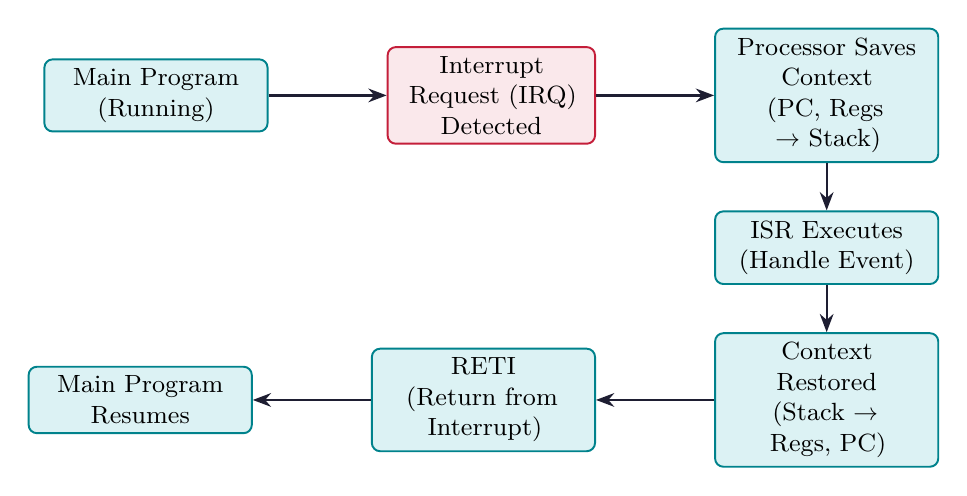
\begin{tikzpicture}[node distance=0.4cm and 1.0cm,
  sblock/.style={rectangle, draw=myteal, fill=hdrteal, text width=2.6cm,
    align=center, minimum height=0.8cm, font=\small, rounded corners=3pt, line width=0.7pt}]
  \node[sblock] (main) {Main Program\\(Running)};
  \node[redblock, right=1.5cm of main] (irq) {Interrupt\\Request (IRQ)\\Detected};
  \node[sblock, right=1.5cm of irq] (save) {Processor Saves\\Context\\(PC, Regs $\to$ Stack)};
  \node[sblock, below=0.6cm of save] (isr) {ISR Executes\\(Handle Event)};
  \node[sblock, below=0.6cm of isr] (rest) {Context\\Restored\\(Stack $\to$ Regs, PC)};
  \node[sblock, left=1.5cm of rest] (ret) {RETI\\(Return from\\Interrupt)};
  \node[sblock, left=1.5cm of ret] (resume) {Main Program\\Resumes};

  \draw[arrow] (main) -- (irq);
  \draw[arrow] (irq) -- (save);
  \draw[arrow] (save) -- (isr);
  \draw[arrow] (isr) -- (rest);
  \draw[arrow] (rest) -- (ret);
  \draw[arrow] (ret) -- (resume);
\end{tikzpicture}
\end{tcolorbox}

\subsection{8051 Interrupt Sources}

The 8051 has \textbf{5 interrupt sources} with a fixed priority:

\par\noindent
{\renewcommand{\arraystretch}{1.55}%
\begin{tabularx}{\linewidth}{|B{3.0cm}|Y|Y|Y|}
\hline
\textbf{Interrupt} & \textbf{Source} & \textbf{Vector Address} & \textbf{Priority (Default)} \\
\hline
\textbf{INT0} & External Pin P3.2 & 0003H & Highest (1) \\
\hline
\textbf{Timer 0} & Timer 0 overflow & 000BH & 2 \\
\hline
\textbf{INT1} & External Pin P3.3 & 0013H & 3 \\
\hline
\textbf{Timer 1} & Timer 1 overflow & 001BH & 4 \\
\hline
\textbf{Serial} & UART TI or RI flag & 0023H & Lowest (5) \\
\hline
\end{tabularx}}

\subsection{Different Interrupt Sources (General)}
\begin{itemize}[leftmargin=*, itemsep=3pt]
  \item \textbf{External Interrupts:} Triggered by a signal change on a pin (edge-triggered or level-triggered).
  \item \textbf{Timer Interrupts:} Triggered when a timer/counter register overflows.
  \item \textbf{Communication Interrupts:} Triggered when UART receives a byte, or SPI transfer completes.
  \item \textbf{ADC Interrupts:} Triggered when analog-to-digital conversion is complete.
  \item \textbf{Software Interrupts (SWI):} Triggered by executing a special instruction (used in ARM for system calls).
  \item \textbf{Reset:} Non-maskable; forces processor to restart (highest priority).
\end{itemize}

% ===============================================================================
\section{Multiple Interrupts, Interrupt Latency and Deadline}
% ===============================================================================

\subsection{Multiple Interrupt Handling}

When several interrupts occur simultaneously, the system must resolve priority:

\begin{itemize}[leftmargin=*, itemsep=3pt]
  \item \textbf{Fixed Priority:} Each interrupt has a fixed, pre-assigned priority level. Higher priority ISR always preempts lower priority (8051 default behavior via IP register).
  \item \textbf{Nested Interrupts:} A higher-priority interrupt can interrupt a currently-executing lower-priority ISR. Requires saving the lower ISR's state on the stack.
  \item \textbf{Interrupt Masking:} Individual interrupts can be enabled/disabled via IE (Interrupt Enable) register bits to prevent interference during critical code sections.
\end{itemize}

\begin{tcolorbox}[masonbox, title={\textbf{8051 Interrupt Enable (IE) Register}}]
\renewcommand{\arraystretch}{1.3}
\begin{tabularx}{\linewidth}{|>{\centering\arraybackslash}X|>{\centering\arraybackslash}X|>{\centering\arraybackslash}X|>{\centering\arraybackslash}X|>{\centering\arraybackslash}X|>{\centering\arraybackslash}X|>{\centering\arraybackslash}X|>{\centering\arraybackslash}X|}
\hline
\textbf{EA} & --- & --- & \textbf{ES} & \textbf{ET1} & \textbf{EX1} & \textbf{ET0} & \textbf{EX0} \\
\hline
Bit 7 & 6 & 5 & 4 & 3 & 2 & 1 & 0 \\
\hline
\end{tabularx}
EA = Global enable; ES = Serial; ET1 = Timer1; EX1 = INT1; ET0 = Timer0; EX0 = INT0
\end{tcolorbox}

\subsection{Interrupt Latency}

\begin{tcolorbox}[defbox, title={\textbf{Interrupt Latency}}]
\textbf{Interrupt latency} is the time elapsed from when an interrupt signal is asserted to when the first instruction of the ISR begins executing. It includes: detecting the interrupt, completing the current instruction, saving context (pushing to stack), and fetching the ISR vector.
\end{tcolorbox}

\begin{tcolorbox}[formulabox, title={\textbf{Interrupt Latency Components}}]
\[
t_{latency} = t_{detect} + t_{inst\_complete} + t_{context\_save} + t_{vector\_fetch}
\]
\begin{itemize}[leftmargin=*, itemsep=2pt, topsep=4pt]
  \item $t_{detect}$: Time for hardware to sample and recognize the interrupt signal.
  \item $t_{inst\_complete}$: Time to finish the currently executing instruction (worst case: longest instruction).
  \item $t_{context\_save}$: Time to push PC (and registers, if applicable) to stack.
  \item $t_{vector\_fetch}$: Time to read the ISR address from the vector table and jump.
\end{itemize}
\textbf{ARM Cortex-M:} Typical latency = 12 clock cycles (with zero wait-state memory).
\end{tcolorbox}

\subsection{Interrupt Deadline}

\begin{tcolorbox}[defbox, title={\textbf{Interrupt Deadline}}]
An \textbf{interrupt deadline} is the maximum allowable time from interrupt occurrence to completion of the ISR response. In \textbf{hard real-time} systems, if the ISR does not complete its critical actions before the deadline, the system fails (e.g., missing a motor control pulse, losing a data byte from UART buffer).
\end{tcolorbox}

\[
t_{latency} + t_{ISR\_execution} \leq t_{deadline}
\]

\textbf{Design rule:} Always keep ISR code as \textbf{short as possible}. Use a flag variable in the ISR and do heavy processing in the main loop (``deferred processing'' or ``bottom half'' approach).

% ===============================================================================
% MANDATORY QUICK REVISION PAGE
% ===============================================================================
\newpage
\begin{center}
  {\large\bfseries\color{myred} Quick Revision --- Module 3}\\[3pt]
  {\small\color{mydark} I/O Types \& Interrupt Service Mechanism $|$ PE-EC703A}
\end{center}
\noindent{\color{myred}\rule{\linewidth}{1.2pt}}
\vspace{4pt}

\begin{tcolorbox}[formulabox, title={\textbf{Key Formulas at a Glance}}]
\renewcommand{\arraystretch}{1.3}
\begin{tabularx}{\linewidth}{B{4.5cm} X}
UART Baud Rate (8051) & $\text{Baud} = \displaystyle\frac{f_{osc}}{32 \times 12 \times (256 - \text{TH1})}$ \\[4pt]
Timer Delay (Mode 1) & $t_{delay} = (65536 - \text{Init\_Count}) \times \displaystyle\frac{12}{f_{osc}}$ \\[4pt]
Interrupt Deadline & $t_{latency} + t_{ISR} \leq t_{deadline}$ \\[4pt]
RTC Crystal Freq & $f = 32768\,\text{Hz} = 2^{15}\,\text{Hz}$ (15-bit counter, 1 overflow/second)
\end{tabularx}
\end{tcolorbox}

\begin{tcolorbox}[defbox, title={\textbf{One-Line Definitions}}]
\begin{itemize}[leftmargin=*, itemsep=2.5pt, topsep=0pt]
  \item \textbf{UART:} Asynchronous serial protocol using start/stop bits; configurable baud rate.
  \item \textbf{I2C:} 2-wire synchronous serial bus (SDA + SCL); multi-master, 7-bit addressing.
  \item \textbf{CAN:} 2-wire differential serial bus for automotive/industrial; message-ID arbitration.
  \item \textbf{ISA:} Legacy 8/16-bit parallel expansion bus from IBM PC (1981); obsolete.
  \item \textbf{Timer:} Hardware counter that counts internal clock pulses to measure time.
  \item \textbf{Counter:} Hardware timer counting external event pulses.
  \item \textbf{WDT:} Watchdog Timer --- resets MCU if software fails to kick it periodically.
  \item \textbf{RTC:} Real-Time Clock --- tracks date and time using 32.768 kHz crystal and coin-cell battery.
  \item \textbf{Interrupt:} Hardware/software signal that suspends main program to run ISR.
  \item \textbf{ISR:} Interrupt Service Routine --- short function handling the interrupt event.
  \item \textbf{Interrupt Latency:} Delay from interrupt request to first ISR instruction.
  \item \textbf{Interrupt Deadline:} Maximum allowable time for ISR to complete its response.
  \item \textbf{NVIC:} ARM's Nested Vectored Interrupt Controller; handles up to 240 priority-based interrupts.
\end{itemize}
\end{tcolorbox}

\begin{tcolorbox}[exambox, title={\textbf{Frequently Asked / Viva Questions}}]
\begin{enumerate}[topsep=0pt, label=\textbf{Q\arabic*.}, itemsep=5pt]
  \item \Q{What is the difference between serial and parallel communication?}
    Serial sends data one bit at a time (fewer wires, longer distance). Parallel sends multiple bits simultaneously (more wires, faster but short-distance only).
  \item \Q{What is UART? Describe its frame format.}
    UART is Universal Asynchronous Receiver/Transmitter. Frame: \textbf{Start bit} (1 bit, low) + \textbf{Data} (5--9 bits, LSB first) + \textbf{Parity bit} (optional) + \textbf{Stop bit(s)} (1 or 2 bits, high). Both ends agree on baud rate; no clock wire.
  \item \Q{What are the two wires in I2C and what do they do?}
    \textbf{SDA} (Serial Data Line): carries data bidirectionally. \textbf{SCL} (Serial Clock Line): carries the synchronization clock generated by the master. Both are open-drain with pull-up resistors.
  \item \Q{Why is CAN used in automobiles instead of I2C or UART?}
    CAN uses differential signaling which is immune to electromagnetic noise. It supports multi-master arbitration (priority-based, non-destructive), reliable error detection (CRC, ACK, bit stuffing), and distances up to 1 km at 50 kbps --- all essential in a noisy vehicle environment.
  \item \Q{What is a Watchdog Timer? Why is it important?}
    A WDT is a hardware timer that resets the MCU if software fails to periodically reset it. It is critical in embedded systems because it provides autonomous recovery from software hangs, infinite loops, or crashes --- without human intervention.
  \item \Q{What is the purpose of the 32.768 kHz crystal in an RTC?}
    32.768 kHz $= 2^{15}$ Hz. A 15-bit counter driven at this frequency overflows exactly once every second, providing a precise 1-second tick for timekeeping without complex division logic.
  \item \Q{Define interrupt latency and list its components.}
    Interrupt latency is the time from interrupt assertion to ISR start. Components: interrupt detection time + current instruction completion time + context save time (PC/regs to stack) + vector table fetch time.
  \item \Q{What is a vector table in embedded systems?}
    A vector table is a fixed memory location (e.g., 0x00000000 in ARM) that stores the starting addresses (vectors) of all ISRs. When an interrupt occurs, the CPU reads the corresponding vector and jumps to the ISR.
  \item \Q{How does the 8051 handle two simultaneous interrupts?}
    The 8051 uses a fixed priority scheme. INT0 has the highest priority and Serial has the lowest. If two interrupts occur simultaneously, the higher-priority one is serviced first. Priority can also be adjusted using the IP (Interrupt Priority) register to create two priority levels.
  \item \Q{What is the difference between edge-triggered and level-triggered interrupts?}
    \textbf{Edge-triggered:} ISR fires on signal transition (rising or falling edge). Responds to event occurrence. \textbf{Level-triggered:} ISR fires as long as the signal remains at the active level. The ISR keeps being called until the condition is cleared.
  \item \Q{Why should an ISR be kept as short as possible?}
    Long ISRs increase interrupt latency for other interrupts, can miss deadlines, may cause data loss (e.g., UART buffer overflow), and increase system unpredictability. Heavy processing should be deferred to the main loop using a flag set by the ISR.
  \item \Q{What is the Timer Mode 2 in 8051 and why is it used for baud rate generation?}
    Mode 2 is an 8-bit auto-reload mode where TL counts from the reload value (stored in TH) to 255 and overflows. On overflow, TL is automatically reloaded from TH. This creates a precise, continuous periodic interrupt --- ideal for generating UART baud rates without software intervention.
\end{enumerate}
\end{tcolorbox}

\begin{tcolorbox}[tikzbox, title={Serial Communication Protocols at a Glance}]
\par\noindent
{\renewcommand{\arraystretch}{1.55}%
\begin{tabularx}{\linewidth}{|B{2.5cm}|Y|Y|Y|Y|}
\hline
\textbf{Protocol} & \textbf{Wires} & \textbf{Speed} & \textbf{Masters} & \textbf{Typical Use} \\
\hline
\textbf{UART} & 2 (TX, RX) & 115.2 kbps typical & 1 & Debug console, GPS \\
\hline
\textbf{SPI} & 4 (MOSI, MISO, SCK, CS) & Up to 50 Mbps & 1 & Flash memory, LCD \\
\hline
\textbf{I2C} & 2 (SDA, SCL) & Up to 3.4 Mbps & Multiple & Sensors, EEPROM \\
\hline
\textbf{CAN} & 2 (CAN-H, CAN-L) & Up to 1 Mbps & Multi-master & Automotive ECU \\
\hline
\textbf{USB} & 4 (D+, D--, VCC, GND) & Up to 10 Gbps & 1 host & PC peripherals \\
\hline
\end{tabularx}}
\end{tcolorbox}


% -- Module 4 -----------------------------------------------------------------
\modulestart{4}{Assembly Language Programming (ALP) in Embedded Systems}

\section{Assembly Language Programming (ALP) in Embedded Systems}
% ===============================================================================

\begin{tcolorbox}[defbox, title={\textbf{Assembly Language Programming (ALP)}}]
\textbf{Assembly language} is a low-level programming language that uses \textbf{mnemonics} (symbolic names for machine instructions) to directly control processor hardware. Each assembly instruction maps one-to-one to a machine code instruction. An \textbf{assembler} translates ALP source code to binary machine code.
\end{tcolorbox}

\subsection{Why ALP is Used in Embedded Systems}
\begin{itemize}[leftmargin=*, itemsep=3pt]
  \item \textbf{Maximum hardware control:} Direct access to all registers, flags, and ports.
  \item \textbf{Tight timing:} Exact instruction cycle count known --- essential for time-critical routines (e.g., bit-bang communication, delay loops).
  \item \textbf{Minimum code size:} No compiler overhead; only absolutely necessary code is generated.
  \item \textbf{Boot code / startup:} Initial stack setup, clock configuration, and interrupt vector setup must be in assembly.
  \item \textbf{ISR optimization:} Critical ISRs are often hand-coded in assembly to minimize latency.
\end{itemize}

\subsection{8051 ALP --- Key Instructions}

\par\noindent
{\renewcommand{\arraystretch}{1.55}%
\begin{tabularx}{\linewidth}{|B{3.0cm}|Y|Y|}
\hline
\textbf{Instruction} & \textbf{Syntax / Example} & \textbf{Description} \\
\hline
\textbf{MOV} & \texttt{MOV A, \#55H} & Move immediate data to accumulator \\
\hline
\textbf{ADD} & \texttt{ADD A, R0} & Add R0 to Accumulator (A = A + R0) \\
\hline
\textbf{SUBB} & \texttt{SUBB A, R1} & Subtract R1 and Carry from A \\
\hline
\textbf{SETB / CLR} & \texttt{SETB P1.0} & Set/clear a specific bit \\
\hline
\textbf{JMP / SJMP} & \texttt{SJMP LOOP} & Unconditional short jump \\
\hline
\textbf{JZ / JNZ} & \texttt{JZ DONE} & Jump if accumulator is zero / not zero \\
\hline
\textbf{DJNZ} & \texttt{DJNZ R2, LOOP} & Decrement R2; jump if not zero (loop control) \\
\hline
\textbf{LCALL / RET} & \texttt{LCALL DELAY} & Long call subroutine / Return from subroutine \\
\hline
\textbf{RETI} & \texttt{RETI} & Return from interrupt (restores context) \\
\hline
\end{tabularx}}

\begin{tcolorbox}[examplebox, title={\textbf{8051 ALP Example: LED Toggle on Port 1}}]
\begin{verbatim}
  ORG  0000H        ; Program start address
  MOV  A, #0FFH     ; Load 0xFF into Accumulator (all bits high)
MAIN:
  MOV  P1, A        ; Send Accumulator to Port 1 (all LEDs ON)
  ACALL DELAY       ; Call 1-second delay subroutine
  CPL  A            ; Complement Accumulator (0xFF -> 0x00)
  SJMP MAIN         ; Repeat forever

DELAY:
  MOV  R0, #0FFH    ; Outer loop: 255 iterations
D1: MOV  R1, #0FFH  ; Inner loop: 255 iterations
D2: DJNZ R1, D2     ; Decrement R1; loop until zero
  DJNZ R0, D1       ; Decrement R0; loop until zero
  RET               ; Return from subroutine
  END
\end{verbatim}
\end{tcolorbox}

% ===============================================================================
\section{High-Level Language Programming --- C for Embedded}
% ===============================================================================

\begin{tcolorbox}[defbox, title={\textbf{C Language for Embedded Systems}}]
\textbf{C} is the dominant high-level language for embedded systems programming. It provides a good balance between \textbf{hardware access} (via pointers, bitwise operations, volatile keyword) and \textbf{productivity} (structured code, functions, libraries). The C code is compiled by a cross-compiler for the target architecture.
\end{tcolorbox}

\subsection{Key C Concepts for Embedded Programming}

\subsubsection*{Volatile Keyword}
\texttt{volatile} tells the compiler that a variable's value can change at any time (e.g., by hardware or an ISR) and must not be cached in a register or optimized away:
\begin{center}
\texttt{volatile uint8\_t flag = 0; \quad // Set by ISR, read by main loop}
\end{center}

\subsubsection*{Bitwise Operations}
Essential for setting, clearing, and testing individual bits in hardware registers:

\par\noindent
{\renewcommand{\arraystretch}{1.55}%
\begin{tabularx}{\linewidth}{|B{3.0cm}|Y|Y|}
\hline
\textbf{Operation} & \textbf{C Code} & \textbf{Effect} \\
\hline
\textbf{Set a bit} & \texttt{reg |= (1 << n)} & Sets bit $n$ without affecting others \\
\hline
\textbf{Clear a bit} & \texttt{reg \&= \~{}(1 << n)} & Clears bit $n$ without affecting others \\
\hline
\textbf{Toggle a bit} & \texttt{reg \^{}= (1 << n)} & Toggles bit $n$ \\
\hline
\textbf{Test a bit} & \texttt{if (reg \& (1 << n))} & Reads state of bit $n$ \\
\hline
\end{tabularx}}

\subsection{Processor Directives in Embedded C}

\begin{tcolorbox}[defbox, title={\textbf{Processor Directives}}]
\textbf{Processor directives} (also called \textbf{preprocessor directives}) are instructions to the C preprocessor that run before actual compilation. They begin with \texttt{\#} and control how the source code is processed.
\end{tcolorbox}

\par\noindent
{\renewcommand{\arraystretch}{1.55}%
\begin{tabularx}{\linewidth}{|B{3.0cm}|Y|Y|}
\hline
\textbf{Directive} & \textbf{Syntax} & \textbf{Purpose} \\
\hline
\textbf{\#define} & \texttt{\#define LED\_PIN 5} & Macro substitution; defines a constant or code snippet \\
\hline
\textbf{\#include} & \texttt{\#include "stm32f4xx.h"} & Includes a header file (device register definitions) \\
\hline
\textbf{\#ifdef / \#endif} & \texttt{\#ifdef DEBUG ... \#endif} & Conditional compilation (include code only for debug builds) \\
\hline
\textbf{\#pragma} & \texttt{\#pragma once} & Compiler-specific directive (prevent double-inclusion) \\
\hline
\textbf{\#ifndef} & \texttt{\#ifndef \_HEADER\_H} & Include guard to prevent multiple inclusions \\
\hline
\end{tabularx}}

\subsection{Functions and Macros in Embedded C}
\begin{itemize}[leftmargin=*, itemsep=3pt]
  \item \textbf{Functions:} Reusable code blocks. Function calls add overhead (stack push/pop of parameters and return address). For embedded systems, frequently called short functions can be declared \texttt{inline} to avoid this overhead.
  \item \textbf{Macros:} Defined with \texttt{\#define}. Expanded inline by the preprocessor --- zero runtime overhead. Used for hardware register bit manipulation, delays, and port pin aliases.
\end{itemize}

\begin{tcolorbox}[examplebox, title={\textbf{C Macro vs.\ Inline Function Example}}]
\begin{verbatim}
/* Macro -- no type safety, zero overhead */
#define SET_BIT(reg, bit)   ((reg) |= (1U << (bit)))
#define CLEAR_BIT(reg, bit) ((reg) &= ~(1U << (bit)))

/* Inline function -- type-safe, zero overhead (compiler expands inline) */
static inline void gpio_set(volatile uint32_t *reg, uint8_t bit) {
    *reg |= (1U << bit);
}

/* Usage */
SET_BIT(GPIOA->ODR, 5);     /* Macro: sets PA5 */
gpio_set(&GPIOB->ODR, 3);   /* Inline function: sets PB3 */
\end{verbatim}
\end{tcolorbox}

\subsection{Embedded C++ Concept}

\begin{tcolorbox}[defbox, title={\textbf{Embedded C++ (EC++)}}]
\textbf{Embedded C++} is a subset of C++ designed for resource-constrained embedded targets. It uses C++ features that add \textbf{zero or minimal overhead} while providing better code organization and type safety compared to plain C.
\end{tcolorbox}

\textbf{C++ features commonly used in embedded:}
\begin{itemize}[leftmargin=*, itemsep=3pt]
  \item \textbf{Classes and Objects:} Encapsulate peripheral drivers (e.g., a \texttt{UART} class with \texttt{send()} and \texttt{receive()} methods).
  \item \textbf{Namespaces:} Prevent name collisions between libraries (e.g., \texttt{hal::uart::init()}).
  \item \textbf{Templates:} Generic, type-safe containers and algorithms (e.g., ring buffer template).
  \item \textbf{Constexpr:} Compile-time constant evaluation reduces runtime overhead.
  \item \textbf{RAII (Resource Acquisition Is Initialization):} Automatic resource management (locks released when object goes out of scope --- critical for RTOS mutexes).
\end{itemize}

\textbf{C++ features AVOIDED in embedded (high overhead):}
\begin{itemize}[leftmargin=*, itemsep=2pt]
  \item Exceptions (\texttt{try}/\texttt{catch}) --- adds large overhead and unpredictable timing.
  \item Runtime Type Information (RTTI) / \texttt{dynamic\_cast} --- requires type tables at runtime.
  \item \texttt{new}/\texttt{delete} (dynamic heap allocation) --- causes fragmentation and non-deterministic timing.
\end{itemize}

% ===============================================================================
\section{Real-Time Operating System (RTOS)}
% ===============================================================================

\begin{tcolorbox}[defbox, title={\textbf{RTOS --- Real-Time Operating System}}]
An \textbf{RTOS} is an operating system designed for \textbf{deterministic, time-bound execution} of tasks. It provides task scheduling, inter-task communication (queues, semaphores, mutexes), memory management, and timer services. Unlike general-purpose OS, an RTOS guarantees task completion within defined time limits.
\end{tcolorbox}

\subsection{OS Overview and Process Management}

\begin{tcolorbox}[formulabox, title={\textbf{RTOS Services}}]
\begin{itemize}[leftmargin=*, itemsep=3pt]
  \item \textbf{Task (Thread) Management:} Create, delete, suspend, resume tasks with different priorities.
  \item \textbf{Scheduling:} Algorithm that decides which task runs on the CPU at any given time.
  \item \textbf{Inter-Task Communication (IPC):} Queues (FIFO data), semaphores (signaling), mutexes (shared resource protection).
  \item \textbf{Memory Management:} Static or dynamic allocation of memory blocks to tasks.
  \item \textbf{Timers:} Software timers for periodic callbacks without a dedicated hardware timer.
  \item \textbf{Examples:} FreeRTOS, Zephyr, RTEMS, VxWorks, uC/OS-II, ThreadX.
\end{itemize}
\end{tcolorbox}

\subsection{RTOS Task States}

\begin{tcolorbox}[tikzbox, title={RTOS Task State Diagram}]
\centering
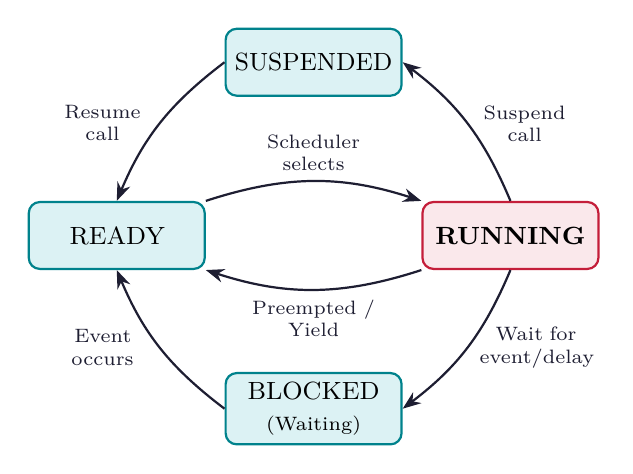
\begin{tikzpicture}[
  tstate/.style={rectangle, draw=myteal, fill=hdrteal, text width=2.0cm,
    align=center, minimum height=0.85cm, font=\small, rounded corners=4pt, line width=0.8pt},
  rstate/.style={rectangle, draw=myred, fill=hdrred, text width=2.0cm,
    align=center, minimum height=0.85cm, font=\small\bfseries, rounded corners=4pt, line width=0.8pt}]

  \node[tstate] (ready)     at (0,   0)    {READY};
  \node[rstate] (running)   at (5,   0)    {RUNNING};
  \node[tstate] (blocked)   at (2.5, -2.2) {BLOCKED \\ \scriptsize(Waiting)};
  \node[tstate] (suspended) at (2.5,  2.2) {SUSPENDED};

  \draw[arrow] (ready.north east) to[bend left=18]
    node[above, font=\scriptsize, align=center] {Scheduler \\ selects} (running.north west);
  \draw[arrow] (running.south west) to[bend left=18]
    node[below, font=\scriptsize, align=center] {Preempted / \\ Yield} (ready.south east);
  \draw[arrow] (running.south) to[bend left=15]
    node[right, font=\scriptsize, align=center, text width=1.5cm] {Wait for \\ event/delay} (blocked.east);
  \draw[arrow] (blocked.west) to[bend left=15]
    node[left, font=\scriptsize, align=center, text width=1.2cm] {Event \\ occurs} (ready.south);
  \draw[arrow] (running.north) to[bend right=15]
    node[right, font=\scriptsize, align=center, text width=1.2cm] {Suspend \\ call} (suspended.east);
  \draw[arrow] (suspended.west) to[bend right=15]
    node[left, font=\scriptsize, align=center, text width=1.2cm] {Resume \\ call} (ready.north);
\end{tikzpicture}
\end{tcolorbox}


\subsection{Task Scheduling Algorithms}

\subsubsection*{1. Priority-Based Preemptive Scheduling}

\begin{tcolorbox}[defbox, title={\textbf{Priority-Based Preemptive Scheduling}}]
Each task is assigned a \textbf{priority} (numeric value). The scheduler always runs the highest-priority task that is in the READY state. If a higher-priority task becomes ready while a lower-priority task runs, the lower-priority task is \textbf{immediately preempted} (stopped) and the higher-priority task takes the CPU.
\end{tcolorbox}

\begin{itemize}[leftmargin=*, itemsep=3pt]
  \item \textbf{Deterministic:} Highest-priority tasks always respond within bounded time.
  \item \textbf{Starvation risk:} Very low-priority tasks may never run if higher-priority tasks are always ready.
  \item \textbf{Priority Inversion:} A high-priority task is blocked because a low-priority task holds a shared resource. Solved by \textbf{Priority Inheritance Protocol}.
  \item \textbf{Used in:} FreeRTOS, VxWorks, RTEMS, most industrial RTOS.
\end{itemize}

\subsubsection*{2. Cyclic Scheduling (Time-Division Multiplexing)}

\begin{tcolorbox}[defbox, title={\textbf{Cyclic Scheduling}}]
Tasks are arranged in a \textbf{fixed cyclic sequence} (also called a \textbf{static schedule}). A major cycle (hypercycle) is divided into \textbf{time slots}, and each task runs during its assigned slot. No dynamic priority decisions --- the schedule is fixed at design time.
\end{tcolorbox}

\begin{itemize}[leftmargin=*, itemsep=3pt]
  \item \textbf{Predictable:} Exact execution times are known at compile time.
  \item \textbf{Simple:} No complex scheduler overhead.
  \item \textbf{Inflexible:} Cannot respond to dynamic events; hard to add new tasks.
  \item \textbf{Used in:} Safety-critical aerospace and automotive systems (ARINC 653, AUTOSAR).
\end{itemize}

\subsubsection*{3. Round-Robin Scheduling}

\begin{tcolorbox}[defbox, title={\textbf{Round-Robin Scheduling}}]
All tasks of \textbf{equal priority} are given equal CPU time \textbf{time slices} (quantum, e.g., 10 ms). The scheduler cycles through all ready tasks in a circular queue. When a task's time slice expires, it is preempted and the next task in the queue runs.
\end{tcolorbox}

\begin{itemize}[leftmargin=*, itemsep=3pt]
  \item \textbf{Fair:} All equal-priority tasks share CPU time equally.
  \item \textbf{No starvation} for equal-priority tasks.
  \item \textbf{Response time:} Depends on the number of tasks and the time quantum (worst case: $(n-1) \times Q$).
  \item \textbf{Used in:} Linux time-sharing, RTOS task groups at same priority.
\end{itemize}

\subsection{Comparison of RTOS Scheduling Algorithms}

\par\noindent
{\renewcommand{\arraystretch}{1.55}%
\begin{tabularx}{\linewidth}{|B{3.0cm}|Y|Y|Y|}
\hline
\textbf{Feature} & \textbf{Priority-Based} & \textbf{Cyclic} & \textbf{Round-Robin} \\
\hline
\textbf{Flexibility} & High & Low & Medium \\
\hline
\textbf{Determinism} & High & Very High & Medium \\
\hline
\textbf{Fairness} & Low (priority skew) & Fixed & High (equal priority) \\
\hline
\textbf{Overhead} & Medium & Very Low & Low \\
\hline
\textbf{Starvation} & Possible & No & No (equal priority) \\
\hline
\textbf{Best For} & General RTOS & Safety-critical & Time-sharing tasks \\
\hline
\end{tabularx}}

\subsection{Basic Design Rules Using RTOS}
\begin{enumerate}[label=\textbf{\arabic*.}, leftmargin=*, itemsep=4pt]
  \item \textbf{Assign priorities carefully:} Critical, fast-response tasks (e.g., motor control) get the highest priority. Background tasks (e.g., logging) get the lowest.
  \item \textbf{Use semaphores/mutexes} to protect shared resources (global variables, hardware peripherals) from concurrent access by multiple tasks.
  \item \textbf{Avoid blocking calls in high-priority tasks:} Use non-blocking APIs or timeouts.
  \item \textbf{Minimize stack usage:} Each task has its own stack. Over-allocating wastes RAM; under-allocating causes stack overflow (hard to debug).
  \item \textbf{Keep ISRs minimal:} ISR sets a flag or sends to a queue; task processes the data.
  \item \textbf{Use RTOS trace tools:} Tools like FreeRTOS+Trace or Segger SystemView to observe task switching, timing, and CPU usage.
\end{enumerate}

% ===============================================================================
% MANDATORY QUICK REVISION PAGE
% ===============================================================================
\newpage
\begin{center}
  {\large\bfseries\color{myred} Quick Revision --- Module 4}\\[3pt]
  {\small\color{mydark} Embedded Software Development \& RTOS $|$ PE-EC703A}
\end{center}
\noindent{\color{myred}\rule{\linewidth}{1.2pt}}
\vspace{4pt}

\begin{tcolorbox}[formulabox, title={\textbf{Key Formulas at a Glance}}]
\renewcommand{\arraystretch}{1.3}
\begin{tabularx}{\linewidth}{B{4.5cm} X}
8051 Delay Loop Cycles & $N_{cycles} = (\text{count}_{outer}) \times (\text{count}_{inner}) \times 5$ (approx., per DJNZ) \\[4pt]
RTOS Response Time (RR) & $t_{response} \leq (n - 1) \times Q$ \quad ($n$ = tasks at same priority, $Q$ = time quantum) \\[4pt]
CPU Utilization Check & $U = \displaystyle\sum_{i=1}^{n} \frac{C_i}{T_i} \leq 1$ \quad ($C_i$ = exec. time, $T_i$ = period of task $i$)
\end{tabularx}
\end{tcolorbox}

\begin{tcolorbox}[defbox, title={\textbf{One-Line Definitions}}]
\begin{itemize}[leftmargin=*, itemsep=2.5pt, topsep=0pt]
  \item \textbf{ALP:} Assembly Language Programming --- low-level mnemonic-based programming for direct hardware control.
  \item \textbf{Assembler:} Translates assembly (mnemonic) code to binary machine code.
  \item \textbf{Cross-compiler:} Compiler on a host PC generating code for a different target (e.g., ARM GCC).
  \item \textbf{volatile:} C keyword that prevents compiler from caching a variable that can change externally (e.g., ISR flag).
  \item \textbf{Preprocessor Directive:} Instructions beginning with \texttt{\#} that control compilation before the compiler runs.
  \item \textbf{Inline function:} C++ function expanded at call site by the compiler, eliminating function call overhead.
  \item \textbf{RTOS:} Operating system guaranteeing deterministic task scheduling with hard timing deadlines.
  \item \textbf{Task (Thread):} An independent unit of execution managed by the RTOS scheduler.
  \item \textbf{Preemption:} RTOS forcibly stopping a running task to run a higher-priority task.
  \item \textbf{Semaphore:} RTOS signaling mechanism for synchronization between tasks or between ISR and tasks.
  \item \textbf{Mutex:} Mutual exclusion object; protects shared resources from concurrent access (includes priority inheritance).
  \item \textbf{Priority Inversion:} A high-priority task blocked by a low-priority task holding a needed resource.
  \item \textbf{Round-Robin:} Scheduling algorithm giving equal time slices to all tasks at the same priority level.
\end{itemize}
\end{tcolorbox}

\begin{tcolorbox}[exambox, title={\textbf{Frequently Asked / Viva Questions}}]
\begin{enumerate}[topsep=0pt, label=\textbf{Q\arabic*.}, itemsep=5pt]
  \item \Q{What is the difference between assembly language and C for embedded programming?}
    ALP gives maximum hardware control, exact cycle-count timing, and minimum code size but is processor-specific and harder to maintain. C provides portability, structured code, and faster development with slightly larger code. Both are commonly mixed: C for application logic, ALP for startup and timing-critical routines.
  \item \Q{What is the purpose of the \texttt{volatile} keyword in embedded C?}
    It tells the compiler that a variable can change unexpectedly (by an ISR, DMA, or hardware register) and must not be optimized or cached. Without \texttt{volatile}, the compiler may read the variable once and reuse the cached value, missing updates.
  \item \Q{What are preprocessor directives? Give two examples.}
    Instructions beginning with \texttt{\#} that are processed before compilation. Examples: \texttt{\#define LED 5} (macro constant), \texttt{\#include "stm32.h"} (file inclusion), \texttt{\#ifdef DEBUG} (conditional compilation).
  \item \Q{What is an RTOS and how does it differ from a bare-metal embedded system?}
    An RTOS provides multi-tasking, scheduling, and synchronization services. In bare-metal, a single \texttt{while(1)} loop and ISRs handle everything sequentially --- no time guarantees between events. RTOS ensures tasks run within defined deadlines and can run concurrently.
  \item \Q{Explain priority-based preemptive scheduling.}
    Each task has a priority number. The RTOS scheduler always runs the highest-priority READY task. If a higher-priority task becomes ready (e.g., unblocked by an ISR posting to its queue), the currently running lower-priority task is immediately preempted and the higher-priority task takes the CPU.
  \item \Q{What is priority inversion and how is it solved?}
    Priority inversion: a high-priority task (H) is blocked waiting for a resource held by a low-priority task (L), while a medium-priority task (M) runs and prevents L from completing. \textbf{Solution:} Priority Inheritance --- temporarily raise L's priority to H's level until it releases the resource.
  \item \Q{Compare cyclic scheduling and round-robin scheduling.}
    Cyclic scheduling uses a fixed time-division slot sequence (fully deterministic, best for safety-critical systems, inflexible). Round-robin dynamically gives equal time quantum to all equal-priority tasks (fair, flexible, slight unpredictability in deadline, good for general tasks).
  \item \Q{What is the difference between a semaphore and a mutex?}
    A \textbf{semaphore} is a signaling mechanism (binary or counting) primarily used for task synchronization and ISR-to-task signaling. A \textbf{mutex} (Mutual Exclusion) is specifically for protecting shared resources from concurrent access and includes priority inheritance to prevent priority inversion.
  \item \Q{What is the role of the RTOS kernel?}
    The RTOS kernel manages task creation, deletion, scheduling (context switching), inter-task communication (queues, semaphores), timers, and memory allocation. It runs the context switch code that saves and restores task registers during task switching.
  \item \Q{What are the advantages of C++ over C in embedded programming?}
    C++ provides encapsulation (classes for peripheral drivers), type safety (templates), compile-time computation (constexpr), and RAII for automatic resource management. These improve code organization and reliability with zero runtime cost if high-overhead features (exceptions, RTTI, heap) are avoided.
  \item \Q{What is a time quantum in round-robin scheduling?}
    The time quantum (slice) is the maximum CPU time a task runs before being preempted and the next task getting a turn. Shorter quantum gives better responsiveness but more context-switch overhead. Typical values: 1--20 ms.
  \item \Q{What is the \texttt{DJNZ} instruction in 8051 assembly and why is it used?}
    \texttt{DJNZ Rn, label} --- Decrement Register $n$ and Jump if Not Zero. It is the standard loop instruction: \texttt{MOV R0, \#100; LOOP: DJNZ R0, LOOP} creates a 100-iteration delay loop with a 2-machine-cycle instruction --- very efficient for timing loops.
\end{enumerate}
\end{tcolorbox}

\begin{tcolorbox}[tikzbox, title={RTOS Scheduling: Priority-Based vs.\ Round-Robin Timeline}]
\centering
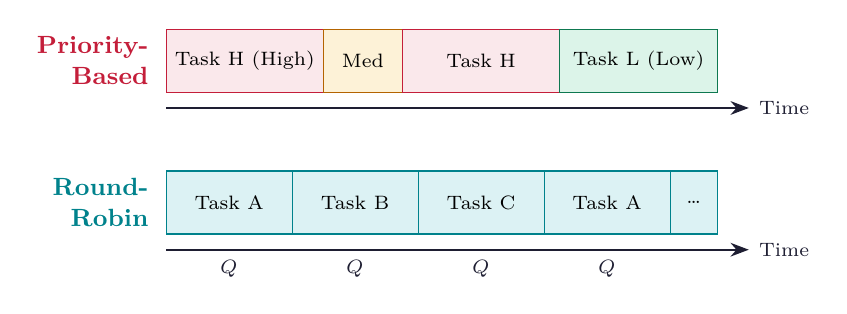
\begin{tikzpicture}[every node/.style={font=\small}]
  % ── Priority-Based row (y = 2.2 – 3.0) ──
  \node[left, align=right, font=\small\bfseries\color{myred}] at (2.5, 2.6) {Priority-\\Based};
  \draw[fill=hdrred,   draw=myred]   (2.6, 2.2) rectangle (4.6, 3.0) node[midway, font=\scriptsize] {Task H (High)};
  \draw[fill=hdramber, draw=myamber] (4.6, 2.2) rectangle (5.6, 3.0) node[midway, font=\scriptsize] {Med};
  \draw[fill=hdrred,   draw=myred]   (5.6, 2.2) rectangle (7.6, 3.0) node[midway, font=\scriptsize] {Task H};
  \draw[fill=hdrgreen, draw=mygreen] (7.6, 2.2) rectangle (9.6, 3.0) node[midway, font=\scriptsize] {Task L (Low)};
  \draw[-Stealth, color=mydark, thick] (2.6, 2.0) -- (10.0, 2.0) node[right, font=\scriptsize] {Time};

  % ── Round-Robin row (y = 0.4 – 1.2) ──
  \node[left, align=right, font=\small\bfseries\color{myteal}] at (2.5, 0.8) {Round-\\Robin};
  \draw[fill=hdrteal, draw=myteal] (2.6, 0.4) rectangle (4.2, 1.2) node[midway, font=\scriptsize] {Task A};
  \draw[fill=hdrteal, draw=myteal] (4.2, 0.4) rectangle (5.8, 1.2) node[midway, font=\scriptsize] {Task B};
  \draw[fill=hdrteal, draw=myteal] (5.8, 0.4) rectangle (7.4, 1.2) node[midway, font=\scriptsize] {Task C};
  \draw[fill=hdrteal, draw=myteal] (7.4, 0.4) rectangle (9.0, 1.2) node[midway, font=\scriptsize] {Task A};
  \draw[fill=hdrteal, draw=myteal] (9.0, 0.4) rectangle (9.6, 1.2) node[midway, font=\scriptsize] {\ldots};
  \draw[-Stealth, color=mydark, thick] (2.6, 0.2) -- (10.0, 0.2) node[right, font=\scriptsize] {Time};
  % Q markers at each slot boundary
  \foreach \x in {3.4, 5.0, 6.6, 8.2} {
    \node[below, font=\scriptsize, color=mydark] at (\x, 0.2) {$Q$};
  }
\end{tikzpicture}
\end{tcolorbox}


% -- Module 5 -----------------------------------------------------------------
\modulestart{5}{Introduction to Microchip PIC16 Family}

\section{Introduction to Microchip PIC16 Family}
% ===============================================================================

\begin{tcolorbox}[defbox, title={\textbf{PIC Microcontroller}}]
\textbf{PIC} (Peripheral Interface Controller) is a family of microcontrollers manufactured by \textbf{Microchip Technology}. PIC microcontrollers are known for their RISC-based Harvard architecture, a small instruction set ($<$35 instructions for mid-range PIC), low cost, wide voltage range (2.0--5.5 V), and abundant peripheral integration. They are widely used in hobbyist and industrial embedded applications.
\end{tcolorbox}

\subsection{PIC Architecture Classifications}

\par\noindent
{\renewcommand{\arraystretch}{1.6}%
\begin{tabularx}{\linewidth}{|B{3.0cm}|Y|Y|Y|}
\hline
\textbf{Family} & \textbf{Program Word} & \textbf{Data Bus} & \textbf{Examples} \\
\hline
\textbf{PIC10 (Base)} & 12-bit & 8-bit & PIC10F200, PIC10F220 \\
\hline
\textbf{PIC12 (Base)} & 12-bit & 8-bit & PIC12F508, PIC12F675 \\
\hline
\textbf{PIC16 (Mid-range)} & 14-bit & 8-bit & PIC16F84A, PIC16F877A, PIC16F873 \\
\hline
\textbf{PIC18 (Enhanced)} & 16-bit & 8-bit & PIC18F4550, PIC18F452 \\
\hline
\textbf{PIC24 / dsPIC} & 24-bit & 16-bit & dsPIC33, PIC24FJ \\
\hline
\textbf{PIC32} & 32-bit MIPS & 32-bit & PIC32MX, PIC32MZ \\
\hline
\end{tabularx}}

\subsection{Key Architectural Features of PIC Mid-Range (PIC16)}
\begin{itemize}[leftmargin=*, itemsep=3pt]
  \item \textbf{Harvard Architecture:} Separate program (Flash) and data (RAM + SFR) buses.
  \item \textbf{RISC Core:} Only 35 instructions; most execute in 1 instruction cycle (4 clock cycles).
  \item \textbf{Instruction Cycle:} $T_{cy} = 4 / f_{OSC}$ (e.g., at 20 MHz: $T_{cy} = 200\,\text{ns}$).
  \item \textbf{8-bit Working Register (W):} Equivalent to the Accumulator in 8051.
  \item \textbf{File Register Architecture:} All RAM, SFRs, and I/O registers accessed via ``file register'' addresses.
  \item \textbf{Pipelining:} 2-stage pipeline (Fetch + Execute) --- while one instruction executes, the next is fetched.
\end{itemize}

\begin{tcolorbox}[formulabox, title={\textbf{PIC16 Key Formulas}}]
\[
T_{cy} = \frac{4}{f_{OSC}} \qquad (\text{1 instruction cycle} = 4 \text{ clock periods})
\]
\[
\text{Timer0 Overflow Time} = \frac{(256 - \text{TMR0}) \times \text{Prescaler} \times 4}{f_{OSC}}
\]
\[
\text{ADC Resolution} = \frac{V_{REF}}{2^N - 1} \quad (N = 10\text{ bits for PIC16F873})
\]
\[
\text{Baud Rate (UART)} = \frac{f_{OSC}}{64 \times (\text{SPBRG} + 1)} \quad (\text{Low speed mode})
\]
\end{tcolorbox}

% ===============================================================================
\section{PIC16F873 --- Architecture and Features}
% ===============================================================================

\begin{tcolorbox}[defbox, title={\textbf{PIC16F873}}]
The \textbf{PIC16F873} is a 28-pin Flash-based mid-range PIC microcontroller from Microchip. It is a popular choice for educational and industrial embedded designs due to its integrated analog and communication peripherals, Flash programmability, and low power consumption.
\end{tcolorbox}

\subsection{PIC16F873 --- Key Specifications}

\par\noindent
{\renewcommand{\arraystretch}{1.55}%
\begin{tabularx}{\linewidth}{|B{3.5cm}|Y|}
\hline
\textbf{Feature} & \textbf{Specification} \\
\hline
\textbf{Program Memory} & 8 KB Flash (4096 x 14-bit words) \\
\hline
\textbf{Data Memory (RAM)} & 192 bytes SRAM \\
\hline
\textbf{Data EEPROM} & 128 bytes \\
\hline
\textbf{I/O Ports} & PORTA (6 pins), PORTB (8 pins), PORTC (8 pins) = 22 I/O \\
\hline
\textbf{Timers} & Timer0 (8-bit), Timer1 (16-bit), Timer2 (8-bit + PR2) \\
\hline
\textbf{ADC} & 5-channel, 10-bit ADC (AN0--AN4 on PORTA) \\
\hline
\textbf{Serial Ports} & USART (UART/SPI async), MSSP (SPI + I2C) \\
\hline
\textbf{Interrupts} & Up to 13 interrupt sources \\
\hline
\textbf{Clock Speed} & DC to 20 MHz (using external crystal) \\
\hline
\textbf{Supply Voltage} & 2.0 V to 5.5 V \\
\hline
\textbf{Package} & 28-pin PDIP, SOIC, SSOP \\
\hline
\textbf{Watchdog Timer} & Built-in WDT with independent RC oscillator \\
\hline
\end{tabularx}}

\begin{tcolorbox}[tikzbox, title={PIC16F873 Block Diagram}]
\centering
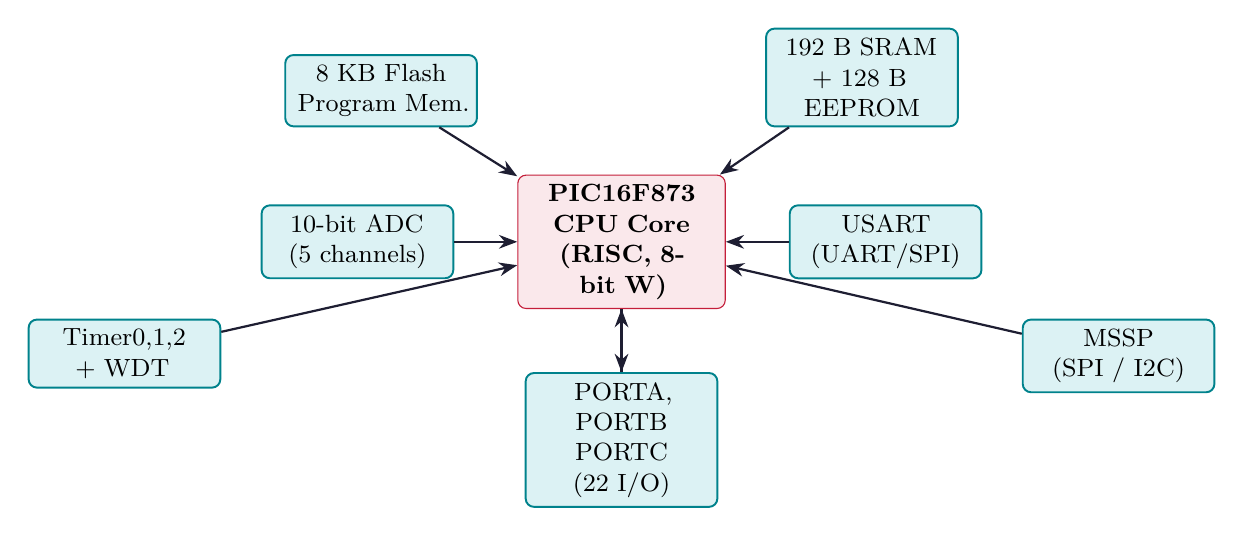
\begin{tikzpicture}[node distance=0.35cm and 0.6cm,
  sblock/.style={rectangle, draw=myteal, fill=hdrteal, text width=2.2cm,
    align=center, minimum height=0.75cm, font=\small, rounded corners=3pt, line width=0.7pt}]
  % Central CPU
  \node[rectangle, draw=myred, fill=hdrred, text width=2.4cm, align=center,
    minimum height=1.0cm, font=\small\bfseries, rounded corners=3pt] (cpu) {PIC16F873\\CPU Core\\(RISC, 8-bit W)};

  % Memory
  \node[sblock, above left=0.6cm and 0.5cm of cpu] (flash) {8 KB Flash\\Program Mem.};
  \node[sblock, above right=0.6cm and 0.5cm of cpu] (sram) {192 B SRAM\\+ 128 B EEPROM};

  % Peripherals left
  \node[sblock, left=0.8cm of cpu] (adc) {10-bit ADC\\(5 channels)};
  \node[sblock, below left=0.5cm and 0.5cm of adc] (tmr) {Timer0,1,2\\+ WDT};

  % Peripherals right
  \node[sblock, right=0.8cm of cpu] (usart) {USART\\(UART/SPI)};
  \node[sblock, below right=0.5cm and 0.5cm of usart] (mssp) {MSSP\\(SPI / I2C)};

  % I/O
  \node[sblock, below=0.8cm of cpu] (io) {PORTA, PORTB\\PORTC (22 I/O)};

  \draw[arrow] (flash) -- (cpu);
  \draw[arrow] (sram) -- (cpu);
  \draw[arrow] (adc) -- (cpu);
  \draw[arrow] (tmr) -- (cpu);
  \draw[arrow] (usart) -- (cpu);
  \draw[arrow] (mssp) -- (cpu);
  \draw[arrow] (io) -- (cpu);
  \draw[arrow] (cpu) -- (io);
\end{tikzpicture}
\end{tcolorbox}

% ===============================================================================
\section{On-Chip Peripherals of PIC16F873}
% ===============================================================================

\subsection{Watchdog Timer (WDT)}
\begin{itemize}[leftmargin=*, itemsep=3pt]
  \item Has its own internal \textbf{RC oscillator} (independent of main clock); continues running even if main clock fails.
  \item Default timeout period $\approx$ 18 ms; extended via \textbf{postscaler} (up to $\times 128$ $\approx$ 2.3 s).
  \item Reset by \texttt{CLRWDT} instruction in software.
  \item On timeout: generates a device reset (MCLR pin goes low momentarily).
  \item Can be enabled/disabled via configuration word bits.
\end{itemize}

\subsection{ADC (Analog-to-Digital Converter)}
\begin{itemize}[leftmargin=*, itemsep=3pt]
  \item \textbf{10-bit successive approximation ADC}: Converts analog voltage to a 10-bit digital value (0 to 1023).
  \item \textbf{5 analog input channels} (AN0--AN4) on PORTA (multiplexed with digital I/O).
  \item \textbf{Reference voltage:} $V_{REF+}$ and $V_{REF-}$ pins (or $V_{DD}$ and $V_{SS}$ by default).
  \item \textbf{Acquisition time:} Capacitor sampling time before conversion starts; minimum 2 $\mu$s.
  \item \textbf{Result format:} Left-justified or right-justified; stored in ADRESH:ADRESL registers.
\end{itemize}

\begin{tcolorbox}[examplebox, title={\textbf{PIC16F873 ADC --- Conversion Steps}}]
\begin{enumerate}[topsep=0pt, leftmargin=*, itemsep=2pt]
  \item Configure ADCON1 (select analog/digital pin assignment and $V_{REF}$).
  \item Configure ADCON0 (select channel AN$x$, clock source, turn ADC ON).
  \item Wait for acquisition time ($\geq 2\,\mu$s).
  \item Set \texttt{GO/DONE} bit in ADCON0 to start conversion.
  \item Poll \texttt{GO/DONE} bit until it clears (conversion complete, $\approx 12 \times T_{AD}$).
  \item Read 10-bit result from \texttt{ADRESH} (high 2 bits) and \texttt{ADRESL} (low 8 bits).
\end{enumerate}
\end{tcolorbox}

\subsection{Asynchronous Serial Port --- USART}
\begin{itemize}[leftmargin=*, itemsep=3pt]
  \item Full-duplex UART on RC6 (TX) and RC7 (RX).
  \item Baud rate controlled by SPBRG register and BRGH bit (high/low speed).
  \item \textbf{High-speed mode (BRGH=1):} $\text{Baud} = f_{OSC} / (16 \times (\text{SPBRG}+1))$
  \item \textbf{Low-speed mode (BRGH=0):} $\text{Baud} = f_{OSC} / (64 \times (\text{SPBRG}+1))$
  \item Interrupt flags: TXIF (transmit buffer empty), RCIF (receive buffer full).
\end{itemize}

\subsection{SPI and I2C --- MSSP Module}
\begin{itemize}[leftmargin=*, itemsep=3pt]
  \item The \textbf{MSSP} (Master Synchronous Serial Port) supports both SPI and I2C modes.
  \item \textbf{SPI Mode:} Uses RC3 (SCK), RC4 (SDI), RC5 (SDO), and any GPIO as CS (Chip Select). Master or slave configurable.
  \item \textbf{I2C Mode:} Uses RC3 (SCL) and RC4 (SDA) with open-drain outputs. Supports 7-bit and 10-bit addressing.
\end{itemize}

% ===============================================================================
\section{Interfacing with PIC16F873}
% ===============================================================================

\subsection{LCD Interfacing}

\begin{tcolorbox}[defbox, title={\textbf{LCD (16$\times$2) Interfacing with PIC16F873}}]
A standard Hitachi HD44780-compatible 16$\times$2 character LCD is interfaced using \textbf{4-bit mode} (4 data lines + 3 control lines) to save I/O pins. Control pins: RS (Register Select: 0=Command, 1=Data), RW (Read/Write, tied to GND for write-only), EN (Enable pulse to latch data).
\end{tcolorbox}

\begin{tcolorbox}[tikzbox, title={PIC16F873 to 16$\times$2 LCD --- 4-bit Interface}]
\centering
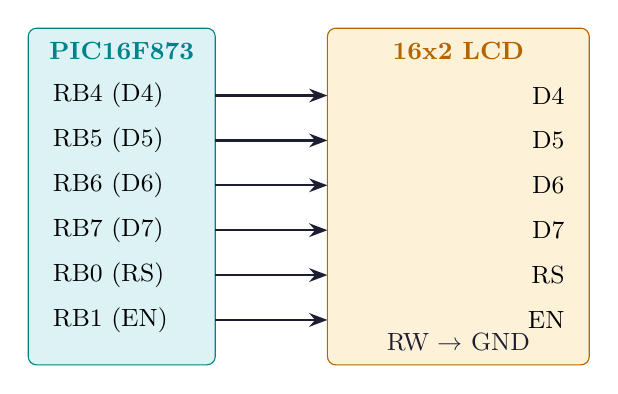
\begin{tikzpicture}[scale=0.95, every node/.style={font=\small}]
  % PIC block
  \draw[fill=hdrteal, draw=myteal, rounded corners=3pt] (0, 0) rectangle (2.5, 4.5);
  \node[font=\small\bfseries, color=myteal] at (1.25, 4.2) {PIC16F873};
  \node[right] at (0.2, 3.6) {RB4 (D4)};
  \node[right] at (0.2, 3.0) {RB5 (D5)};
  \node[right] at (0.2, 2.4) {RB6 (D6)};
  \node[right] at (0.2, 1.8) {RB7 (D7)};
  \node[right] at (0.2, 1.2) {RB0 (RS)};
  \node[right] at (0.2, 0.6) {RB1 (EN)};

  % Connections
  \foreach \y in {3.6, 3.0, 2.4, 1.8, 1.2, 0.6}
    \draw[arrow] (2.5, \y) -- (4.0, \y);

  % LCD block
  \draw[fill=hdramber, draw=myamber, rounded corners=3pt] (4.0, 0) rectangle (7.5, 4.5);
  \node[font=\small\bfseries, color=myamber] at (5.75, 4.2) {16x2 LCD};
  \node[left] at (7.3, 3.6) {D4};
  \node[left] at (7.3, 3.0) {D5};
  \node[left] at (7.3, 2.4) {D6};
  \node[left] at (7.3, 1.8) {D7};
  \node[left] at (7.3, 1.2) {RS};
  \node[left] at (7.3, 0.6) {EN};
  \node[font=\small, color=mydark] at (5.75, 0.3) {RW $\to$ GND};
\end{tikzpicture}
\end{tcolorbox}

\subsection{ADC Interfacing (Sensors)}
\begin{itemize}[leftmargin=*, itemsep=3pt]
  \item Temperature sensor (LM35): Output voltage = 10 mV/$^\circ$C. Connect to AN0.
    \begin{itemize}
      \item ADC result $\to$ Temperature: $T(^{\circ}C) = \frac{\text{ADC} \times V_{REF}}{1023 \times 0.01}$
    \end{itemize}
  \item Potentiometer / Joystick: Directly connected to analog input (voltage divider).
  \item Light sensor (LDR): Used in voltage divider; ADC reads light level.
\end{itemize}

\subsection{Stepper Motor Interfacing}
\begin{itemize}[leftmargin=*, itemsep=3pt]
  \item A stepper motor advances by a fixed angle (step) for each control pulse.
  \item \textbf{Step angle:} Depends on motor type (e.g., $1.8^\circ$/step = 200 steps/revolution).
  \item \textbf{Driver IC:} L298N or ULN2003 connects between PIC output pins and motor coils.
  \item PIC sends sequence of bit patterns to PORTB to rotate the stepper.
  \item \textbf{Full-step sequence (4-phase):} 1100 $\to$ 0110 $\to$ 0011 $\to$ 1001 (repeat).
\end{itemize}

\subsection{Keyboard (Keypad) Interfacing}
\begin{itemize}[leftmargin=*, itemsep=3pt]
  \item A \textbf{4$\times$4 matrix keypad} uses 4 row + 4 column lines = 8 pins.
  \item PIC drives rows LOW one at a time, then reads which column line goes LOW.
  \item The row/column combination identifies the pressed key.
  \item Debouncing: Software delay ($\sim$20 ms) after detecting key press before confirming it.
\end{itemize}

\subsection{DAC (Digital-to-Analog Converter)}
\begin{itemize}[leftmargin=*, itemsep=3pt]
  \item PIC16F873 has no built-in DAC. External options:
    \begin{itemize}
      \item \textbf{R-2R Resistor Ladder:} Passive DAC using resistors connected to PORTB (8-bit). Simple, low cost, no extra IC.
      \item \textbf{External DAC IC (MCP4921):} 12-bit DAC with SPI interface.
      \item \textbf{PWM + RC filter:} Use Timer2 PWM output, filter with RC low-pass $\to$ analog voltage proportional to duty cycle.
    \end{itemize}
\end{itemize}

% ===============================================================================
\section{Case Studies of Embedded System Design}
% ===============================================================================

\subsection{Case Study 1: Automated Chocolate Vending Machine}

\begin{tcolorbox}[examplebox, title={\textbf{Automated Chocolate Vending Machine using PIC16F873}}]
\textbf{Problem:} Design a vending machine that accepts coins (detected by IR sensor), displays balance on LCD, dispenses chocolate (stepper motor) when enough coins are inserted, and provides change.

\textbf{Hardware Components:}
\begin{itemize}[leftmargin=*, itemsep=2pt, topsep=4pt]
  \item PIC16F873 (controller), 16$\times$2 LCD (display), IR coin sensor on AN0 (ADC), Stepper motor + ULN2003 (dispenser), Buzzer on RB0 (feedback), Keypad for item selection.
\end{itemize}

\textbf{Software Flow:}
\begin{enumerate}[topsep=4pt, leftmargin=*, itemsep=2pt]
  \item Initialize LCD, ADC, I/O ports.
  \item Display ``Insert Coin'' on LCD.
  \item Loop: Poll coin sensor (ADC reading $>$ threshold $\to$ coin detected).
  \item On coin: Increment balance; update LCD display.
  \item If balance $\geq$ price: Drive stepper motor (4 steps) to dispense; beep buzzer.
  \item Calculate and dispense change (reverse stepper? No --- separate change mechanism).
  \item Reset balance; display ``Thank You''.
\end{enumerate}

\textbf{Key Programming Concepts Used:} ADC polling, stepper motor control sequences, LCD 4-bit mode, software debounce, timer-based delay.
\end{tcolorbox}

\begin{tcolorbox}[tikzbox, title={Vending Machine System Block Diagram}]
\centering
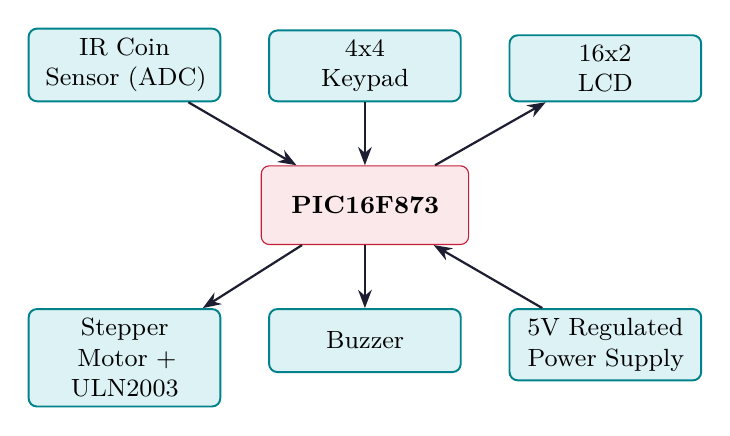
\begin{tikzpicture}[node distance=0.3cm and 0.6cm,
  sblock/.style={rectangle, draw=myteal, fill=hdrteal, text width=2.2cm,
    align=center, minimum height=0.8cm, font=\small, rounded corners=3pt, line width=0.7pt}]
  \node[rectangle, draw=myred, fill=hdrred, text width=2.4cm, align=center,
    minimum height=1.0cm, font=\small\bfseries, rounded corners=3pt] (pic) {PIC16F873};
  \node[sblock, above left=0.8cm and 0.5cm of pic] (coin) {IR Coin\\Sensor (ADC)};
  \node[sblock, above=0.8cm of pic] (keypad) {4x4\\Keypad};
  \node[sblock, above right=0.8cm and 0.5cm of pic] (lcd) {16x2\\LCD};
  \node[sblock, below left=0.8cm and 0.5cm of pic] (motor) {Stepper\\Motor + ULN2003};
  \node[sblock, below=0.8cm of pic] (buzzer) {Buzzer};
  \node[sblock, below right=0.8cm and 0.5cm of pic] (pwr) {5V Regulated\\Power Supply};

  \draw[arrow] (coin) -- (pic);
  \draw[arrow] (keypad) -- (pic);
  \draw[arrow] (pic) -- (lcd);
  \draw[arrow] (pic) -- (motor);
  \draw[arrow] (pic) -- (buzzer);
  \draw[arrow] (pwr) -- (pic);
\end{tikzpicture}
\end{tcolorbox}

\subsection{Case Study 2: Digital Camera Controller}

\begin{tcolorbox}[examplebox, title={\textbf{Digital Camera Controller using PIC (Concept)}}]
\textbf{Note:} A full digital camera uses high-performance processors (e.g., ARM Cortex-A) for image processing. PIC16F873 can implement the \textbf{camera control subsystem} (not image processing).

\textbf{PIC16F873 Role in Digital Camera:}
\begin{itemize}[leftmargin=*, itemsep=2pt, topsep=4pt]
  \item \textbf{Shutter Control:} Timer-based precise shutter speed control (1/1000s to 1/30s) using Timer1 interrupt.
  \item \textbf{Focus Motor Control:} Stepper motor drives lens position; PIC reads ADC from autofocus sensor.
  \item \textbf{Flash Trigger:} GPIO pin triggers external flash unit via optocoupler.
  \item \textbf{User Interface:} Reads mode dial (keypad), displays settings on small LCD.
  \item \textbf{Battery Monitor:} ADC reads battery voltage divider; displays charge level.
  \item \textbf{Serial Communication:} UART or SPI to main image processor (ARM) for command passing.
\end{itemize}

\textbf{Key Techniques:} Timer interrupts for precision timing, ADC for sensor reading, SPI for inter-processor communication, WDT for reliability.
\end{tcolorbox}

% ===============================================================================
% MANDATORY QUICK REVISION PAGE
% ===============================================================================
\newpage
\begin{center}
  {\large\bfseries\color{myred} Quick Revision --- Module 5}\\[3pt]
  {\small\color{mydark} Embedded System Design using PIC Microcontroller $|$ PE-EC703A}
\end{center}
\noindent{\color{myred}\rule{\linewidth}{1.2pt}}
\vspace{4pt}

\begin{tcolorbox}[formulabox, title={\textbf{Key Formulas at a Glance}}]
\renewcommand{\arraystretch}{1.3}
\begin{tabularx}{\linewidth}{B{4.5cm} X}
Instruction Cycle & $T_{cy} = \displaystyle\frac{4}{f_{OSC}}$ \quad (at 20 MHz: $T_{cy} = 200\,\text{ns}$) \\[4pt]
Timer0 Overflow & $t_{TMR0} = \displaystyle\frac{(256 - \text{TMR0\_init}) \times \text{Prescaler} \times 4}{f_{OSC}}$ \\[4pt]
ADC Result (10-bit) & $V_{in} = \displaystyle\frac{\text{ADC} \times V_{REF}}{1023}$ \quad (right-justified) \\[4pt]
UART Baud (BRGH=1) & $\text{Baud} = \displaystyle\frac{f_{OSC}}{16 \times (\text{SPBRG}+1)}$ \\[4pt]
ADC Temperature (LM35) & $T(^{\circ}\text{C}) = \displaystyle\frac{\text{ADC} \times V_{REF}}{1023 \times 0.01}$
\end{tabularx}
\end{tcolorbox}

\begin{tcolorbox}[defbox, title={\textbf{One-Line Definitions}}]
\begin{itemize}[leftmargin=*, itemsep=2.5pt, topsep=0pt]
  \item \textbf{PIC:} Peripheral Interface Controller --- Microchip Technology's RISC-based MCU family.
  \item \textbf{PIC16F873:} 28-pin, 8-bit Flash PIC MCU; 8 KB Flash, 192 B SRAM, 10-bit ADC, USART, MSSP.
  \item \textbf{W Register:} Working Register in PIC --- equivalent to Accumulator; all ALU operations use W.
  \item \textbf{File Register:} PIC's general-purpose RAM + SFR memory, accessed via file register addresses.
  \item \textbf{ADCON0/1:} ADC Control registers in PIC16F873 that configure channel selection, clock, and reference.
  \item \textbf{MSSP:} Master Synchronous Serial Port --- supports SPI and I2C in PIC16F873.
  \item \textbf{USART:} Universal Synchronous/Asynchronous Receiver/Transmitter --- UART + SPI on PIC.
  \item \textbf{SPBRG:} Serial Port Baud Rate Generator register --- sets UART baud rate in PIC.
  \item \textbf{Prescaler:} Divides the clock signal before reaching the timer --- extends the timer overflow period.
  \item \textbf{TMR0:} 8-bit Timer/Counter in PIC16F873 (overflows at 255 $\to$ 0, generates TMR0IF).
  \item \textbf{CLRWDT:} Assembly instruction to reset the Watchdog Timer in PIC.
  \item \textbf{Full-step sequence:} 4-phase stepper motor control pattern (1100, 0110, 0011, 1001).
\end{itemize}
\end{tcolorbox}

\begin{tcolorbox}[exambox, title={\textbf{Frequently Asked / Viva Questions}}]
\begin{enumerate}[topsep=0pt, label=\textbf{Q\arabic*.}, itemsep=5pt]
  \item \Q{What does PIC stand for and who manufactures it?}
    PIC stands for \textbf{Peripheral Interface Controller}. It is manufactured by \textbf{Microchip Technology Inc.}
  \item \Q{State the key features of PIC16F873.}
    28-pin PDIP; 8 KB Flash program memory; 192 B SRAM; 128 B EEPROM; 10-bit 5-channel ADC; three timers (Timer0/1/2); USART; MSSP (SPI + I2C); up to 20 MHz clock; 2.0--5.5 V supply; built-in WDT.
  \item \Q{What is the W register in PIC? How is it different from 8051's Accumulator?}
    The \textbf{W (Working) register} is PIC's primary data register used for ALU operations. Similar to the Accumulator in 8051, it is used as the source/destination for most arithmetic and logic instructions. Unlike 8051's A, W is not directly addressable in the file register map.
  \item \Q{What is the instruction cycle of PIC16 and how does it relate to clock frequency?}
    One instruction cycle = 4 clock cycles: $T_{cy} = 4/f_{OSC}$. At 20 MHz, $T_{cy} = 200\,\text{ns}$. Most PIC instructions execute in 1 cycle (200 ns); branch instructions take 2 cycles.
  \item \Q{How does the PIC16F873 ADC work? What is the resolution?}
    It is a 10-bit successive approximation ADC. It samples the analog voltage on AN0--AN4, converts it to a 10-bit number (0--1023) representing $V_{in}$ between $V_{REF-}$ and $V_{REF+}$. Resolution = $V_{REF}/1023$ (e.g., $\approx 4.88\,\text{mV}$ for 5V reference).
  \item \Q{Explain how a stepper motor is interfaced with PIC16F873.}
    The PIC outputs a 4-bit step sequence to PORTB (e.g., 1100, 0110, 0011, 1001 for full-step mode). Each pattern energizes the motor coils in sequence. A ULN2003 Darlington driver IC between PORTB and the motor coils amplifies the current. The step rate (delay between patterns) controls motor speed.
  \item \Q{What is the difference between USART and MSSP in PIC16F873?}
    \textbf{USART:} Handles asynchronous serial (UART) and synchronous serial (SPI) communication on RC6/RC7. \textbf{MSSP:} A second serial module supporting both SPI (master/slave) and I2C master/slave modes on RC3/RC4/RC5. Both can be used simultaneously.
  \item \Q{How is LCD interfaced with PIC16F873 in 4-bit mode?}
    Only 4 data lines (D4--D7) are connected to PORTB, along with RS and EN control lines (RW tied to GND). Data is sent as two 4-bit nibbles (high nibble first, then low nibble), each latched by pulsing EN high then low.
  \item \Q{How does the Watchdog Timer work in PIC16F873?}
    The WDT has its own RC oscillator ($\approx$18 ms period). Software must execute \texttt{CLRWDT} instruction before timeout. If not cleared in time (e.g., due to program hang), WDT causes a device reset. Timeout can be extended using a postscaler (up to $\times 128 \approx 2.3\,\text{s}$).
  \item \Q{What are the Timer modes available in PIC16F873?}
    \textbf{Timer0:} 8-bit timer/counter with prescaler (1:2 to 1:256). \textbf{Timer1:} 16-bit timer/counter, can use external crystal for low-power RTC. \textbf{Timer2:} 8-bit timer with prescaler and postscaler; period register PR2 sets overflow point; used for PWM generation.
  \item \Q{Describe the design of an automated vending machine using PIC16F873.}
    \begin{itemize}[leftmargin=*, itemsep=1pt, topsep=2pt]
      \item IR sensor (ADC) detects coins; balance tracked in SRAM variable.
      \item LCD (4-bit mode) shows balance and prompts.
      \item Keypad selects product; price compared with balance.
      \item If balance $\geq$ price: stepper motor (via ULN2003) dispenses product; buzzer beeps.
      \item Balance decremented by price; ``Thank You'' displayed.
    \end{itemize}
  \item \Q{Why is PIC preferred for cost-sensitive embedded applications?}
    PIC MCUs are very inexpensive (PIC16F84A $\sim$ Rs.~80--160), available in small packages, have wide voltage range (2--5.5 V), abundant development tools (MPLAB IDE, free compiler), large community, and integrate all needed peripherals on-chip (eliminating external ICs). They are ideal for high-volume, cost-sensitive consumer products.
\end{enumerate}
\end{tcolorbox}

\begin{tcolorbox}[tikzbox, title={PIC16F873 vs.\ 8051 vs.\ ARM Cortex-M0 --- Comparison}]
\par\noindent
{\renewcommand{\arraystretch}{1.55}%
\begin{tabularx}{\linewidth}{|B{2.5cm}|Y|Y|Y|}
\hline
\textbf{Feature} & \textbf{PIC16F873} & \textbf{8051 (AT89S52)} & \textbf{ARM Cortex-M0} \\
\hline
\textbf{Architecture} & Harvard RISC (8-bit) & Harvard CISC (8-bit) & Harvard RISC (32-bit) \\
\hline
\textbf{Instructions} & 35 (14-bit words) & 255 (variable) & Thumb-2 (16/32-bit) \\
\hline
\textbf{Max Clock} & 20 MHz & 33 MHz & 48 MHz \\
\hline
\textbf{Flash} & 8 KB & 8 KB (ISP) & 32--128 KB \\
\hline
\textbf{RAM} & 192 bytes & 256 bytes & 8--32 KB \\
\hline
\textbf{Built-in ADC} & 10-bit, 5-ch & None & 12-bit, 8+ ch \\
\hline
\textbf{Price (approx.)} & Rs.~40--160 & Rs.~65--160 & Rs.~80--400 \\
\hline
\textbf{IDE} & MPLAB X & Keil, SDCC & Keil, GCC ARM \\
\hline
\end{tabularx}}
\end{tcolorbox}


\end{document}
